\documentclass[
	%parspace, % Add vertical space between paragraphs
	%noindent, % No indentation of first lines in each paragraph
	%nohyp, % No hyphenation of words
	%twoside, % Double sided format
	%draft, % Quicker draft compilation without rendering images
	%final, % Set final to hide todos
]{elteikthesis}[2023/04/10]

% The minted package is also supported for source highlighting
% See minted-intregration.tex for example
\usepackage[newfloat]{minted}
\usepackage{url} 

% Document's metadata
\title{Moodle csoportfeladat tevékenységmodul} % title
\date{2024} % year of defense

% Author's metadata
\author{Tóth Botond}
\degree{programtervező informatikus BSc}

% Superivsor(s)' metadata
\supervisor{dr. Nikovits Tibor} % internal supervisor's name
\affiliation{mesteroktató, matematikus} % internal supervisor's affiliation
%\extsupervisor{Külső Kornél} % external supervisor's name
%\extaffiliation{informatikai igazgató} % external supervisor's affiliation

% University's metadata
\university{Eötvös Loránd Tudományegyetem} % university's name
\faculty{Informatikai Kar} % faculty's name
\department{Információs Rendszerek Tanszék} % department's name
\city{Budapest} % city
\logo{elte_cimer_szines} % logo

% Add bibliography file
\addbibresource{elteikthesis.bib}

% The document
\begin{document}

% Set document language
\documentlang{hungarian}

% List of todos (not in the final document)
%\listoftodos[\todolabel]

% Title page (mandatory)
\maketitle
% Topic declaration page (mandatory) - can also be attached instead
%\includepdf{temabejelento.pdf}

% Table of contents (mandatory)
\tableofcontents
\cleardoublepage

% Main content
\chapter{Bevezetés}
\label{ch:intro}

A Moodle napjaink egyik legelterjedtebb nyílt forráskódú elearning keretrendszere. A rendszer nagy előnye, hogy nagyon egyszerűen egészíthető ki segédprogramokkal, így egyedi igényekkel tudjuk a rendszer komponenseit bővíteni anélkül, hogy az eredeti forráskódot módosítanunk kellene. A rendszer lehetőség ad egyedi tevékenységmodulok, beiratkozási lehetőségek vagy akár riportok fejlesztésére. A Moodle-ben minden tevékenységet, minden felhasználó egyedileg old meg, aktív csoportos feladatmegoldásra nincs lehetőség. Szakdolgozatom témája egy egyedi tevékenységmodul\footnote{Tevékenységmodul: A Moodle kurzusainak alkotóelme. Minden kurzus tevékenységmodulokból épül fel, melyeknek különböző tulajdonságai vannak (például Scorm csomag, H5P modul, Kérdőív) } , melyben csoportos feladatmegoldásra van lehetősége a hallgatóknak. 

A modul célja, hogy egy tevékenységen belül valósuljon meg a csoportok és szerepek kiosztása, a csoportokon belüli csevegés, feladat beadása, illetve a feladat értékelése minden csoporttag számára. A segédprogram támogatni fogja a Moodle-ben definiált szerepek használatát, de saját egyedi szerepeket is kioszthatunk a csoportunkon belül.

Ezeken felül a fejlesztés célja, hogy a modul feleljen meg a Moodle keretrendszer konvencióinak és aktívan használja az LMS\footnote{LMS: Learning Management System, elearning keretrendszer} által nyújtott lehetőségeket. Fejlesztésemben nagy hangsúly került a Moodle- integrációra, így számos a rendszer által támogatott plusz funkciót támogat a segédprogram. A fejlesztés alatt egység- és eseményvezérelt tesztelést használtam.

\cleardoublepage

\chapter{Felhasználói dokumentáció}

\label{ch:user}

A tevékenységmodul célja, hogy csoportos feladatokat tudjunk kiadni a hallgatók számára kurzuson belül. A segédprogram telepítése után, "Csoport feladat" típusú modul hozzáadására lesz lehetőségünk minden kurzusban. A modult csak létező kurzuson belül lehet használni és csak az arra jogosult felhasználók tudják majd a kurzushoz hozzáadni.

A modulban hallgatói csoportok létrehozására lesz lehetőségünk, ahol a kurzusba beiratkozott felhasználókat rendelhetjük a tevékenység csoportjaiba. Minden csoporttagsághoz lehetőség nyílik szerep hozzárendelésére, így bizonyos tagoknak többletjogot tudunk adni. A csoporttagok, egy külön felületen képesek szinkron kommunikálni egymással. A feladat beadására egy külön felületen van lehetősége a csoportnak, ahova már a kész munkát kell feltölteni. A feltöltött munkák a Moodle által biztosított fájlkezelő rendszerben kerülnek eltárolásra. Ezeket a munkákat a kurzusba beíratott tanárok láthatják és értékelhetik a modul által biztosított módszer alapján. Az értékelés után a csoport összes tagja megkapja a pontot/értékelést a munkájára és ez a kurzus felültén meg is jelenik.

Az egyedi jogosultságokat és szerepeket csak a portáladminisztrátorok képesek szerkeszteni az arra kijelölt felületen. A modul ezeken felül támogatja még a Moodle által Backup-nak nevezett funkciót, így el tudjuk menteni a tevékenyégünk állapotát és vissza tudjuk az állítani úgy, hogy a benne generálódott adatok perzisztensek maradnak. Moodle Event-ek definiálva vannak a segédprogramon belül, így számos naplózási funkciót támogat a program.

\section{Telepítés}

A program használatához szükséges egy arra megfelelő szerveren telepíteni a Moodle-t. Ehhez szükségünk lesz egy webszerverre, egy adatbáziskezelőre és a PHP egy adott verziójára a szerveren.

\subsection{Rendszerkövetelmények}


A modul megfelelő működéséhez szükséges, hogy az alábbi szoftverek telepítve legyenek a Moodle-t futtató szerveren:

\begin{itemize}
    \item A Moodle verziója: 4.2
    \item A fenti verzióhoz szükséges rendszerkövetelmények:

\begin{itemize}
        \item Webszerver program, például Apache 2.4+ vagy Ngnix 1.24+
        \item PHP verziója: 8.0+
        \item Adatbáziskezelő, például MariaDB 10.6.+ vagy MySQL 8.0+
\end{itemize}

\end{itemize}
Bővebb információ a rendszerkövetelményekről és az ajánlott PHP modulokról a Moodle hivatalos oldalán található.\footnote{\url{https://moodledev.io/general/releases/4.2}}  A verzióhoz tartozó Moodle telepítési utasítások megtalálhatók a hivatalos Moodle dokumentáció telepítési oldalán.\footnote{\url{https://docs.moodle.org/402/en/Installation}} 
 
\subsection{Moodle telepítés}

A Moodle telepítése a webszerver konfigurációja után böngészőből vagy akár parancssorból is megtörténhet. Telepítéshez szükségünk van a Moodle forráskódjára amit a Moodle hivatalos weboldalán\footnote{\url{https://download.moodle.org/releases/supported/}} vagy GitHub repository-ban\footnote{\url{https://github.com/moodle/moodle}} találhatunk meg. 

A sikeres telepítés után a helyes működés érdekében fontos a szerveren a Cron job\footnote{Időzített háttérfolyamat} konfigurációja. Ennek konfigurációjáról a Moodle dokumentációjában találunk bővebb információt.\footnote{\url{https://docs.moodle.org/402/en/Cron}}

\subsection{Segédprogram telepítése}

A segédprogramok telepítése manuálisan és felületről is lehetésges. A telepítést már maga a segédprogram és a Moodle rendszere végzi, telepítés után van lehetőségünk a segédprogram beállításait módosítani.

\subsubsection{\textbf{A telepítés lépései a következők:}}
\begin{compactenum}
	\item A rendszer karbantartási üzemmód bekapcsolása. Így a felhasználók nem érik el a portált a telepítés alatt.
	\item Célszerű biztnosági mentést készíteni a Moodle jelenlegi állapotáról. Ezt adatbázismentéssel, illetve a Moodle számára fenntartott \textit{sitedata} mappa mentésével tudjuk elvégezni.
	\item A segédprogram forráskódjának bemásolása
    \begin{compactitem}
    	\item Manuális másolás esetén a segédprogram forráskódját be kell másolnunk a szerveren az erre fenntartott mappába. A segédprogramunknak van egy típusa, ami arra utal, hogy melyik mappába kell bemásolnunk telepítésnél. Ebben az esetben a \textit{mod} mappába kell elhelyeznünk a segédprogramot.
     \item Felületen történő telepítés esetén fontos, hogy a Moodle-t futtató webszerver felhasználója képes legyen a telepített Moodle \textit{mod} mappájába írni, mivel ide kerül kicsomagolásra a feltöltött modul a rendszer által. A felületen az alábbi URL-en keresztül érjük a manuális telepítést: \url{/admin/tool/installaddon/index.php}. Ide ZIP fájként tudjuk feltölteni a segédprogram forráskódját.
     \end{compactitem}
     \item A bemásolás után felületen megjelenik a portáladminisztrátorok számára a telepítési nézet, itt tudjuk elfogadni a segédprogram telepítését a rendszerünkbe. Ezután a rendszerünk telepíti a segédprogramunkat és elnavigál minket a kezdő oldalra.
     \item Érdemes meggyőződni arról, hogy a program valóban telepítésre került-e. E célból érdemes ellenőrizni az alábbi linket: \url{/mod/groupproject/manage_roles.php}. Ha a link elérhető akkor kikapcsolhatjuk a karbantartási módot és megkezdhetjük az alkalmazás használatát.

\end{compactenum}

\section{Portáladminisztrátor funkciói}

A modul néhány funkciója csak a portáladminisztrátorok számára elérhető. A segédprogram által kezelt szerepköröket csak a portáladminisztrátorok tudják létrehozni és módosítani. Emellett az adminisztrátorok a modul összes jogosultságával rendelkeznek, így ők nem jelennek meg a jogosultság kezelő felületen.

\subsection{Szerepkörök kezelése}

A szerepkörök kezelése oldal a Segédprogramok -> Tevékenységmodulok -> Csoportfeladat -> Szerepkörök kezelése menüpontban érhető el. Kurzusban lévő modul esetén a \textit{Csoportok kezelése} oldalról is elérhető egy link erre az oldalra. Az itt megjelenített szerepkörök a modul által csoporton belül használható szerepeket jeleníti meg létrehozás sorrendjében. Itt az adminisztrátorok képesek új szerepet létrehozni vagy meglévőket módosítani/törölni (Műveletek oszlop). Fontos megjegyezni, hogy ezek a szerepkörök csak a modul által kezelt csoportokra érvényesek. Ezeket a szerepköröket csak a tevékenységmodulon belüli csoportokban lehet használni, rendszerszintű jogosultságokat nem adhatunk velük. A táblázat tartalmazza a szerep nevét, leírását, illetve jogosultságait.

\begin{figure}[H]
	\centering
	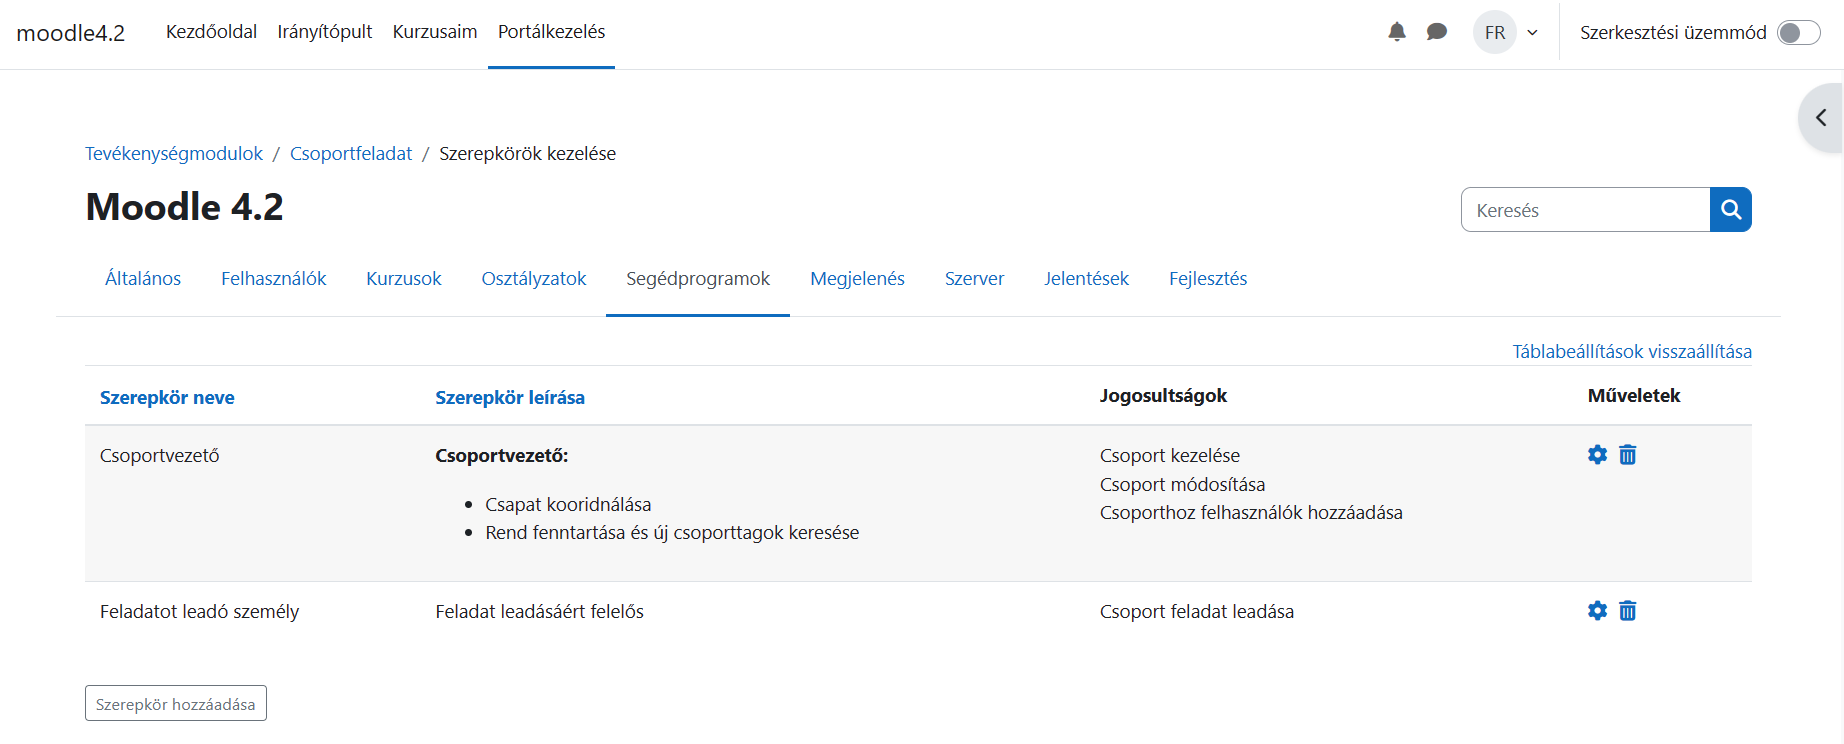
\includegraphics[width=0.8\textwidth,frame]{images/szerepkorok_kezelese.png}
	\caption{Szerepkörök áttekintése}
\end{figure}

\subsection{Szerepkör létrehozása, módosítása és törlése  }

A szerepkörök kezelése menüpontból érhető el az új szerepkör létrehozása opció. Meglévő szerepkör esetén a fogaskerék ikonra kattintva a szerepkör adatait módosíthatjuk. A kuka ikonra kattintás után egy biztonsági ellenőrzés után a szerepkör törlésre kerül. A szerepkör létrehozási és módosítási menüpontban a szerepkör nevét, leírását és jogosultságait adhatjuk meg. A szerepkörnek az elérhető jogosultságok közül akármennyit megadhatunk. Ezek a jogosultságok a tanulóknak csak a csoportjukon belül lesznek elérhetőek. Fontos, hogy a szerepkörünk törlésével a csoportban keletkezett összes felhasználó szerepkör hozzárendelés törlődik, így a törölt szerepkörrel rendelkező csoporttagok innentől szerepkör nélküli tagként fognak viselkedni..

\begin{figure}[H]
	\centering
	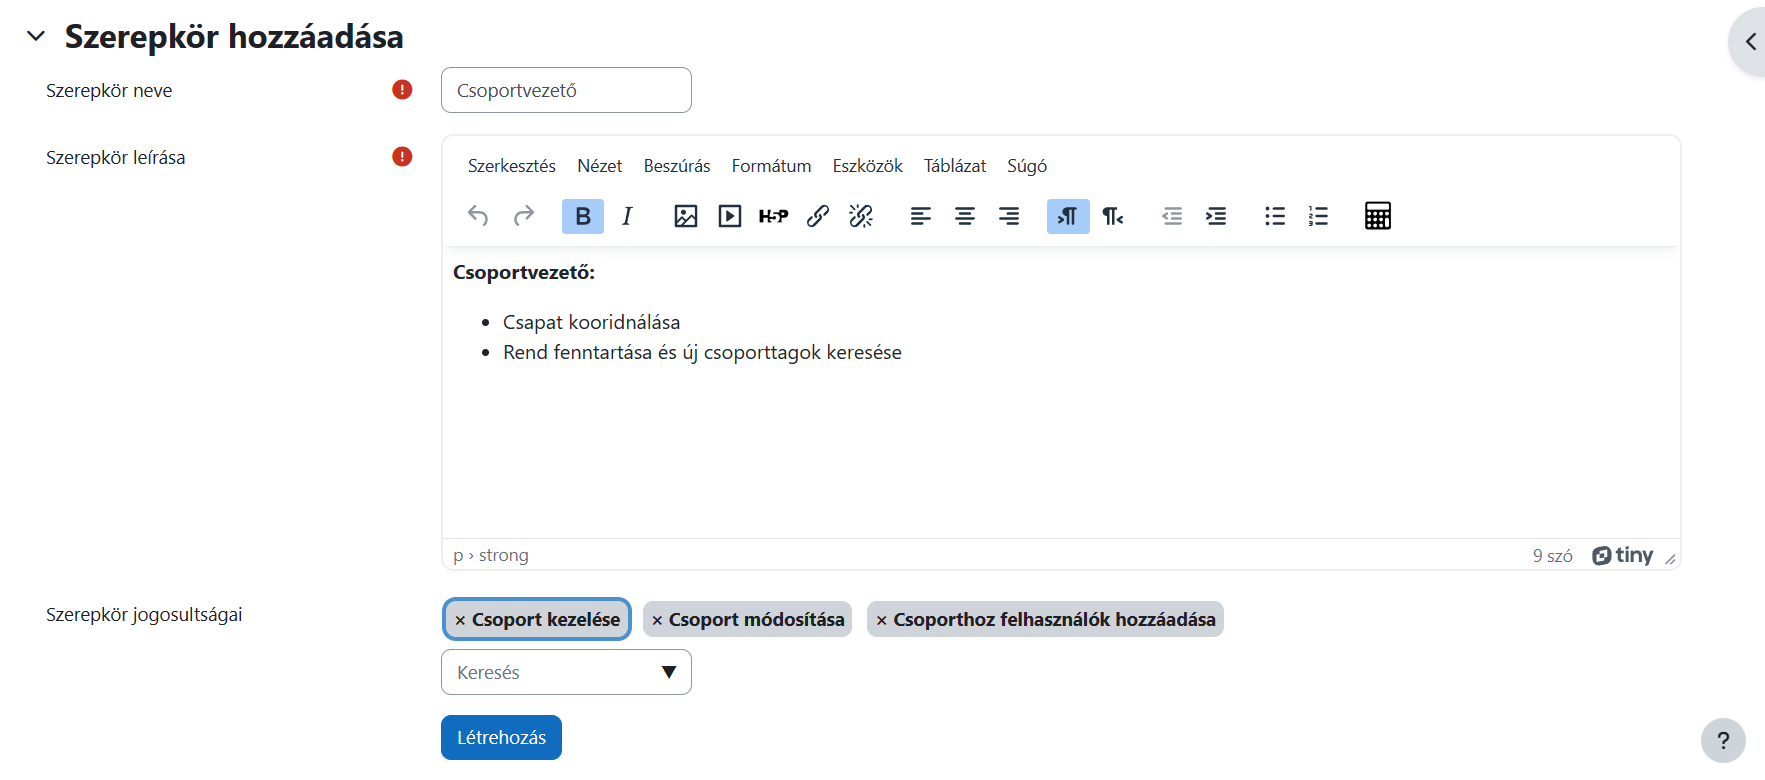
\includegraphics[width=0.8\textwidth,frame]{images/szerepkor_letrehozas.png}
	\caption{Szerepkör létrehozása űrlap}
\end{figure}

\section{Tanárok funkciói}

A segédprogram a tanárok számára adja a legtöbb lehetőséget funkcionalitás terén. A tanárok a kurzuson belüli összes beállítási és konfigurációs felületet elérik, emellett a tevékenységen belül is csoport és feladatszervezési beállításokat tudnak módosítani. Tanárnak az számít, aki a kurzus vagy a tevékenység kontextusában\footnote{Kontextus: Környezet, a Moodle-ben minden oldal rendelekzik egy kontextussal, amin belül többletjogokat adhatunk felhasználóknak.} rendelkezik a \textit{teacher} vagy az \textit{editingteacher} szerepkörrel.

\subsection{Tevékenységmodul kezelése}

Tanárként tudunk a kurzuson belül új tevékenységeket hozzáadni. Itt van lehetőségünk egy új modul típus, a Csoportfeladat kiválasztására. A modul általános beállításain kívül van lehetőségünk pontozási rendszert beállítani a tevékenységünknek. A pontozási rendszer a Moodle által támogatott Skála és Pont alapján történhet. Teljesítési beállításoknál elérhetőek a következő opciók:

\begin{compactitem}
    	\item Tevékenység megtekintése: a felhasználónak elég megnyitni a modult, a teljesítési feltétel a megnyitás pillanatában teljesül.
        \item Osztályzat megszerzése: a felhasználónak szükséges osztályzatot szerezni a teljesítéshez. Az osztályzat eredménye itt nem számít. Érdemes Skála alapú pontozásnál alkalmazni.
        \item Megfelelt osztályzat megszerzése: a felhasználónak szükséges osztályzatot szerezni a teljesítéshez. Az osztályzat eredménye ha alacsonyabb, mint a teljesítéshez megadott pontszám, a felhasználó nem teljesíti a modult. Érdemes Pont alapú pontozásnál alkalmazni.
\end{compactitem}

Ha szeretnénk a kurzus teljesítését értékeléshez kötni, a modulunk minden esetben létrehoz egy pontozási tételt, így a kurzus pontozási riportjában is látható lesz mint új oszlop. A pontozási menün belül, a beadási határidőt is megszabhatjuk, így tudjuk jelezni a hallgatók felé a feladat véghatáridejét.

A tevékenység létrehozása után a modul elérhető lesz a kurzuson belül és lehetőségünk lesz a csoportok létrehozására.

\begin{figure}[H]
	\centering
	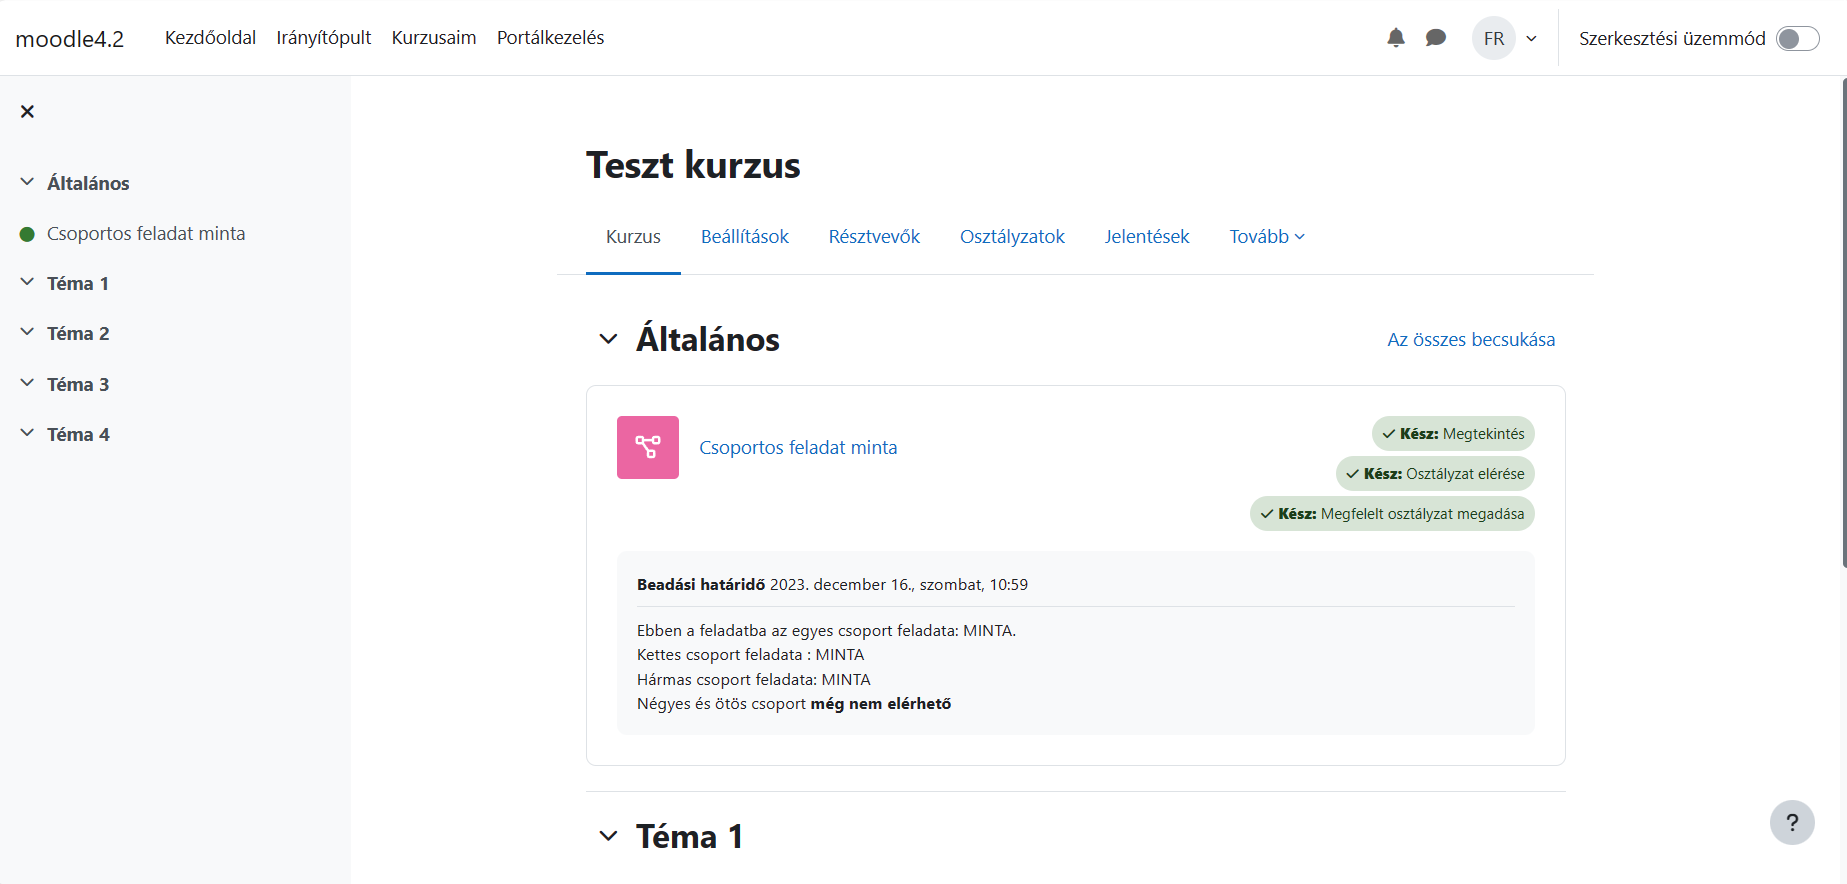
\includegraphics[width=0.8\textwidth,frame]{images/tevekenyseg_nezet.png}
	\caption{Új Csoportfeladat tevékenységmodul a kurzusunkban}
\end{figure}

Mivel a Csoportfeladat támogatja a Moodle Backup funkcióit, így lehetőségünk van a kurzus felületen duplikálni az ilyen típusú kurzusmodulokat. Duplikálásnál felhasználói adatok nem kerülnek át az új tevékenységbe, csak a csoportok és a tevékenység beállításai.

\subsection{Engedélyek kezelése}

Az alkalmazásban a következő egyedi jogosultságok érhetőek el:
\begin{compactitem}
    	\item Csoportmegjegyzés írása: a felhasználó megjegyzést írhat a csoportja csevegésébe. Fontos előfeltétele a jogosultságnak, hogy a felhasználónak rendelkeznie kell csoporttal.
     \item Csoport létrehozása: új csoport létrehozása.
     \item Csoport kezelése: meglévő csoport adatainak módosítása. Hallgatók esetén ez a jogosultság csak saját csoport módosítására ad lehetőséget, ha szerepkörön keresztül került hozzáadásra a jogosultság.
     \item Csoport törlése: meglévő csoport és azzal kapcsolatos összes adat törlése.
     \item Csoporthoz felhasználók hozzáadása: új csoporttagok felvétele a csoportba. Hallgatók esetén ez a jogosultság csak saját csoport módosítására ad lehetőséget, ha szerepkörön keresztül került hozzáadásra a jogosultság.
     \item Csoport értékelése: csoportok értékelése felület elérhetőségét korlátozza.
     \item Csoport feladat leadása: a felhasználó csoportjának leadási felületének elérhetőségét tudjuk vele korlátozni. 
\end{compactitem}

\begin{figure}[H]
	\centering
	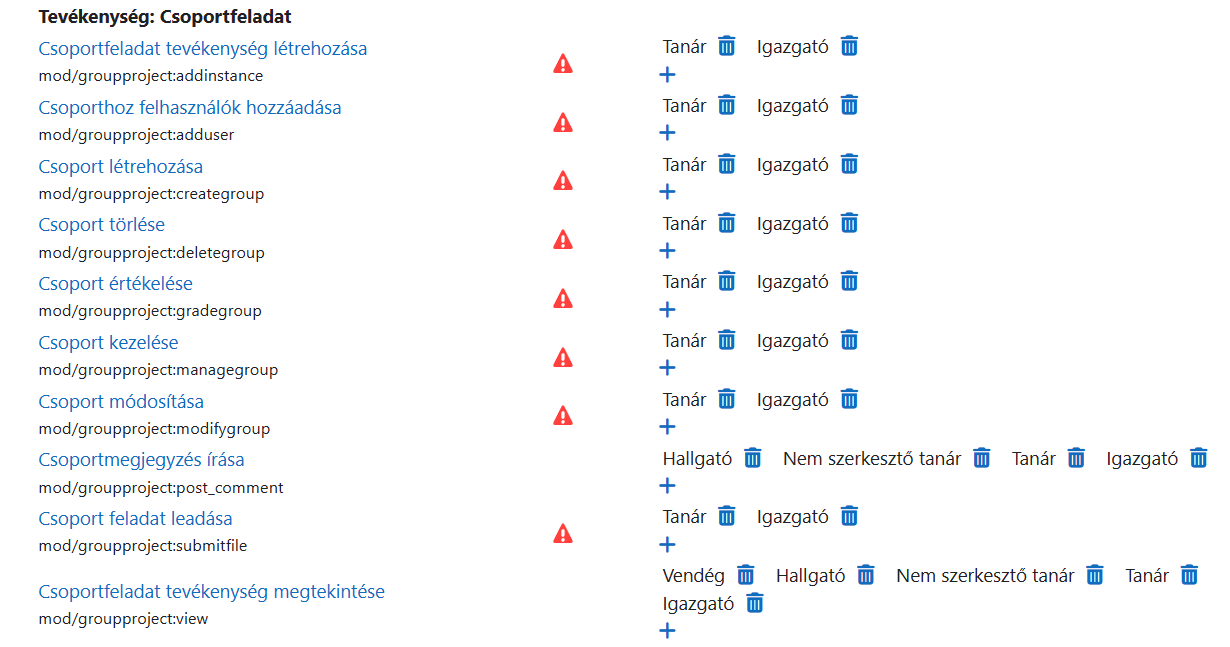
\includegraphics[width=0.8\textwidth,frame]{images/engedelyek.png}
	\caption{Elérhető engedélyek a modulban}
\end{figure}

A jogosultságok, mind tevékenység szinten kerültek definiálásra, így egyedileg módosíthatóak akár kurzuson belül is, ha van két tevékenységünk.

\subsection{Csoportok kezelése}

Ha a tevékenységre kattintunk a tanárok a \textit{Csoportok kezelése }oldalra irányítódnak át. A csoport kezelési felületen a tanárok egy összegző felületet látnak, ahol az eddig létrehozott csoportok találhatóak. Itt tudunk új csoportot létrehozni, meglévőt módosítani vagy akár törölni. A táblázat tartalmazza a csoport nevét, a csoport jelenlegi és maximális létszámát. A csoport által beadott munka is letölthető az oldalról, illetve a csoport által szerzett értékelés is megjelenik a táblázatban. A tanárok megtekinthetik az elérhető szerepköröket (egy linken keresztül), viszont módosítani nem módosíthatják azokat.

\begin{figure}[H]
	\centering
	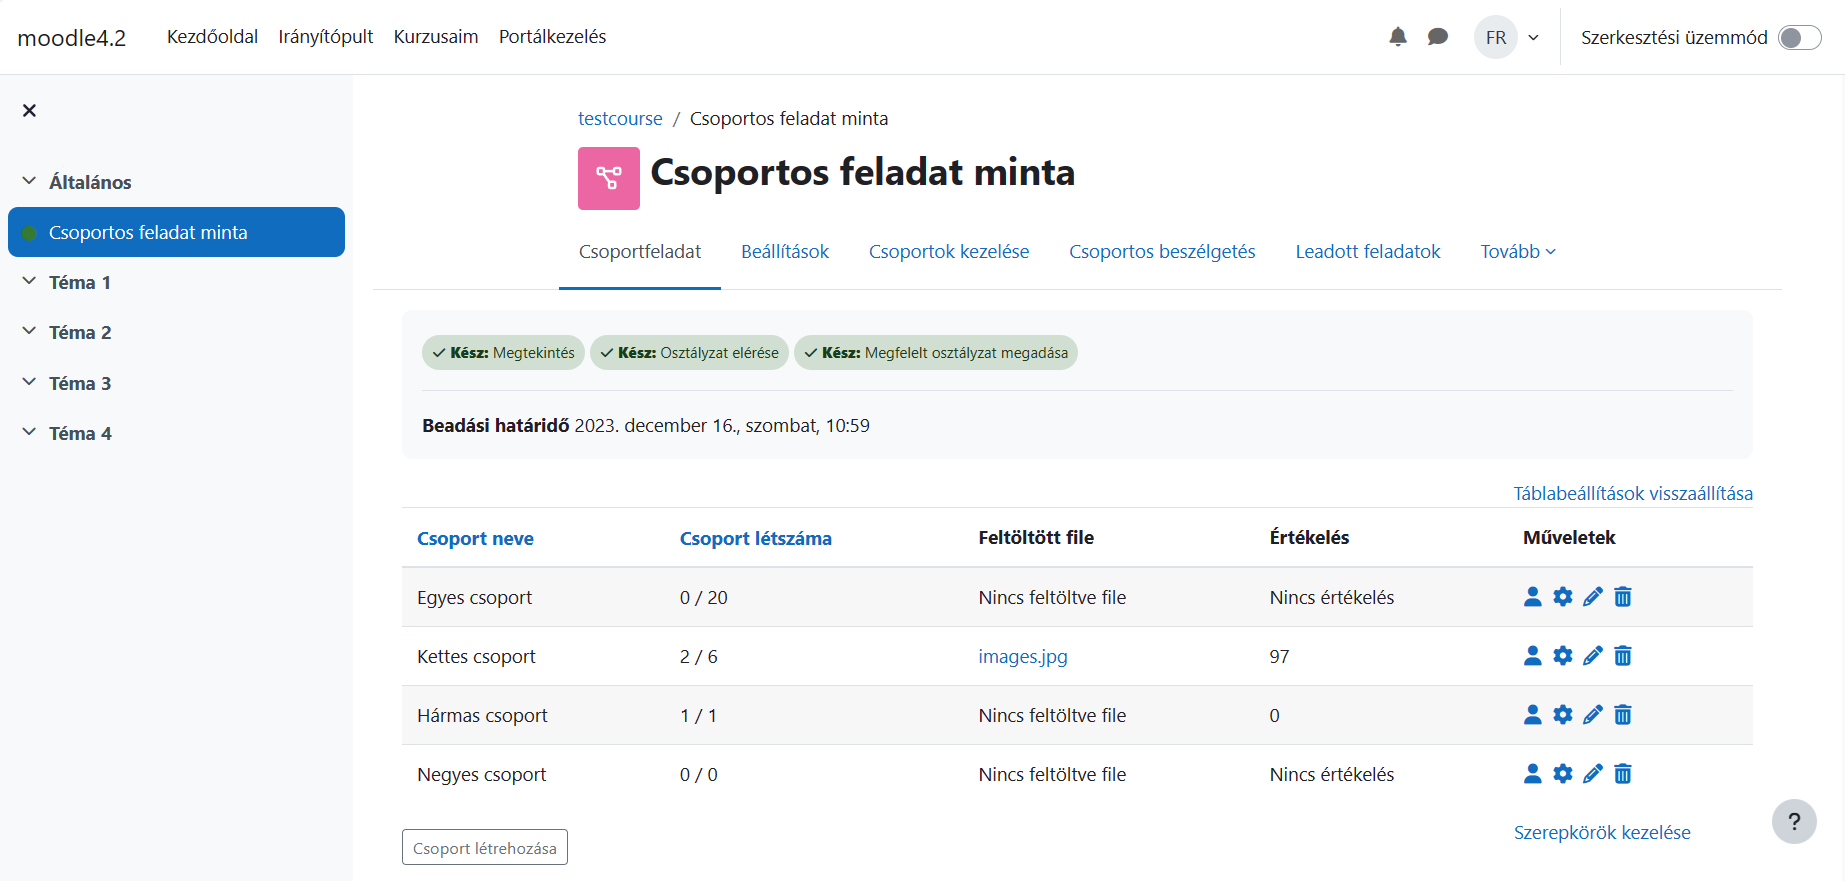
\includegraphics[width=0.8\textwidth,frame]{images/csoportok_kezelese.png}
	\caption{Csoportok kezelése tevékenységmodulban}
\end{figure}

\subsection{Csoport létrehozása, módosítása és törlése}

A csoportok kezelése menüpontból érhető el az új csoport létrehozása opció. Meglévő csoport esetén a fogaskerék ikonra kattintva a csoport adatait módosíthatjuk. A kuka ikonra kattintás után egy biztonsági ellenőrzés után a csoport törlésre kerül. A csoport létrehozási és módosítási menüpontban a csoport nevét, azonosítóját és létszámát adhatjuk meg. A csoportlétszám korlátozni fogja az egyszerre aktív csoporttagok számát. Fontos, hogy a csoportunk törlésével a csoportban keletkezett összes adat törlődik, így a csoport tagjainak üzenetei, fájljai, értékelései mind törlődnek a csoporttal együtt.

\begin{figure}[H]
	\centering
	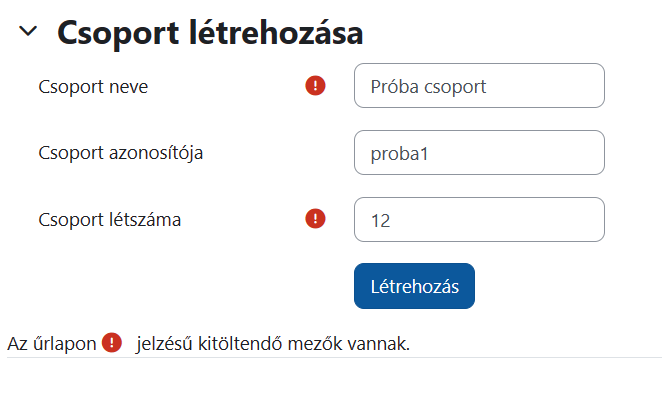
\includegraphics[width=0.8\textwidth,frame]{images/csoport_letrehozas.png}
	\caption{Csoport létrehozása űrlap}
\end{figure}

\subsection{Csoporttagok felvétele}

A csoportok kezelése menüpontból elérhető a csoporttagok felvételi oldala. Meglévő csoport esetén a Műveletek oszlopban található ember ikonra kattintással érhetjük el az oldalt. Ha a csoport nem üres, akkor a meglévő csoporttagok listáját fogjuk látni, a hozzájuk rendelt szerepkörökkel. A csoporttag neve és szerepköre mellett egy kuka ikon is található, amivel ki tudjuk törölni a felhasználót a csoportból. A potenciális felhasználók listáját a segédprogram a kurzusba beíratott felhasználók közül válogatja ki. Olyan felhasználók akik már másik csoport tagjai nem fognak megjelenni a potenciális felhasználók között. Új felhasználó felvételére egészen addig van lehetőségünk még a csoportlétszám be nem telik. Új csoporttagot akár szerepkör nélkül is fel tudunk venni. Az űrlap csak akkor kerül mentésre ha leadjuk azt a Felhasználók hozzáadása gombbal. A törölt felhasználók üzenetei megmaradnak a csoportban, egyéb adatai elvesznek.

\begin{figure}[H]
	\centering
	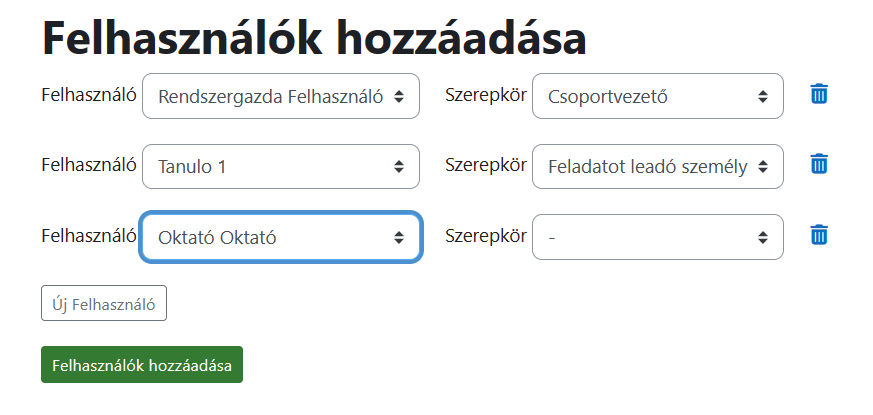
\includegraphics[width=0.8\textwidth,frame]{images/felhasznalok_hozzaadasa.png}
	\caption{Felhasználók hozzáadása űrlap}
\end{figure}

\subsection{Csoportok értékelése}

A modul lehetőséget ad a Moodle által támogatott összes pontozási lehetőségre. A tevékenység létrehozásakor megadott pontozási módszerrel (ha beállításra került) képes a pontozást végző tanár értékelést adni a csoportnak. Ezen módszerek lehetnek Pont, illetve Skála alapúak. Ha pontozás megtörtént, az értékelés a csoportban lévő összes hallgató számára beírásra kerül. A kurzus összegző felületén, az összegző riportban jelenik meg a hallgatók összpontszáma, a modulban kiosztott pontszámok alapján. Az értékelés a csoport összegző felültén is meg fog jelenni.

\begin{figure}[H]
	\centering
	\subcaptionbox{Pontszám alapú eredmény megadása}{
		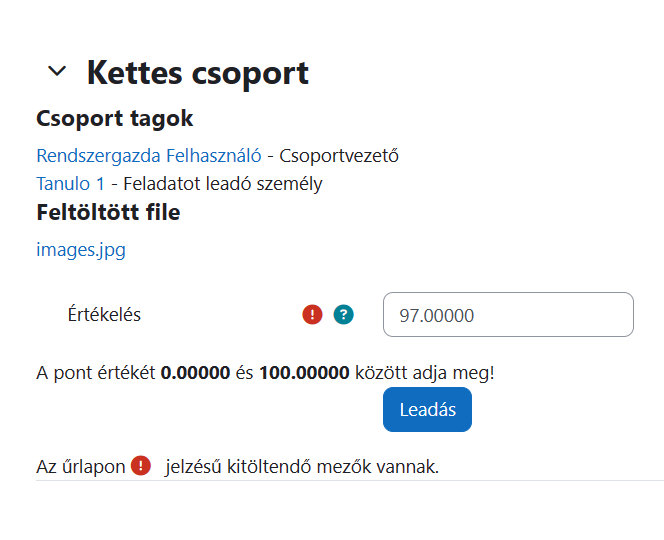
\includegraphics[width=0.45\linewidth,frame]{images/pontszam_pontozas.png}}
	\hspace{5pt}
	\subcaptionbox{Skála alapú pontszám megadása}{
		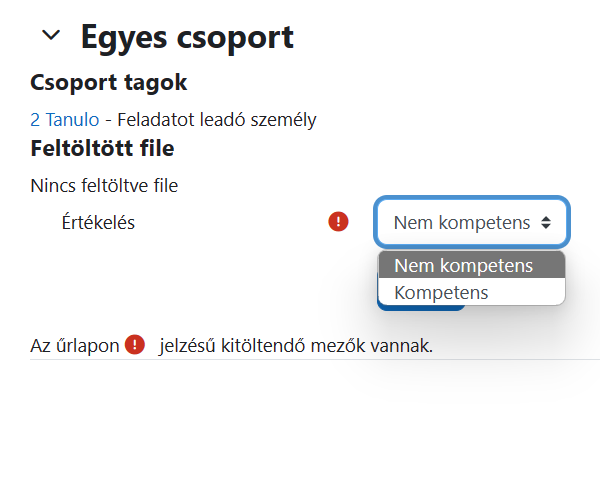
\includegraphics[width=0.45\linewidth,frame]{images/skala_pontozas.png}}
	\caption{Pont és skála alapú értékelés összehasonlítása}
	\label{fig:example-2}
\end{figure}

\subsection{Biztonsági mentés, visszaállítás és importálás funkció}

A Moodle által támogatott \textit{Backup} funkció is támogatott a segédprogramon belül. Tanárként tudunk biztonsági mentést készíteni a tevékenységmodulunk jelenlegi állapotáról. Ezt a biztonsági mentést tárolni fogja a Moodle és lehetőségünk lesz visszaállítani a modult egy régebbi állapotra. A biztonsági mentés nem csak abba a rendszerbe tölthető vissza, ahol a mentés megtörtént. A segédprogramunk által generált adatokat tetszőleges Moodle rendszerbe tudjuk visszatölteni. (persze csak abban az esetben, ha a másik rendszer is rendelkezik a segédprogramunkkal). Az importálás funkció a fent említett két művelet egy időben való végrehajtása: készül egy biztonsági mentés a modulunk állapotáról, majd ezt a biztonsági mentést visszatöltjük egy meglévő vagy új kurzusba. A mentés és importálás során el tudjuk dönteni, hogy a felhasználói adatokat is szeretnénk-e átvinni az új modulba. Fontos, hogy ha ezzel a lehetőséggel nem élünk, akkor a felhasználói csoporthozzárendelések, leadott fájlok, csoportok jegyei illetve a csoportok beszélgetései nem kerülnek migrálásra. 

\section{Hallgatók funkciói}

A hallgatók igazán csak akkor tudják az applikáció adta lehetőségeket kihasználni ha egy csoport tagjai lesznek. A csoporton belül minden hallgatónak lehet egy egyedi szerepe, amit a csoporttagság kezdetekor kapott. Ezekkel a szerepekkel egyes csoporttagoknak többletjogot adhatunk.

\subsection{Csoportos csevegés}

Ha a hallgató egy csoport tagja, a tevékenységre kattintás után rögtön a csoportos beszélgetés menübe kerül, ahol látja az éppen aktív csoportjának csevegését. A beszélgetés szinkron módon történik, így a hallgatók valós időben tudják egymással megosztani a feladat részleteit, illetve a megoldás közben felmerülő problémákat. (A leadott változatában a programban beállításra került egy 8 másodperces késleltetés prezentációs célokból) A csoporttagok profilképei is megjelennek a beszélgetés közben, amire ha a hallgató rákattint, a felhasználó profiloldalára irányítódik át. A beszélgetés üzenetküldésére egy TinyMCE\footnote{TinyMCE: WYSIWYG HTML szerkesztő, \url{https://www.tiny.cloud/tinymce/}} multifunkcionális szerkesztő áll rendelkezésre, mely képes képek, emoji-k, és HTML tartalmak értelemezésére, így az üzenet tartalma lényegében bármi lehet. A beszélgetésben való részvétel is egy jogosultsághoz van kötve, viszont ezzel minden hallgató rendelkezik. A portáladminisztrátorok képesek ezt a jogosultságot elvenni a felhasználótól, ha nem megfelelően kommunikál tanulótársaival.
\begin{figure}[H]
	\centering
	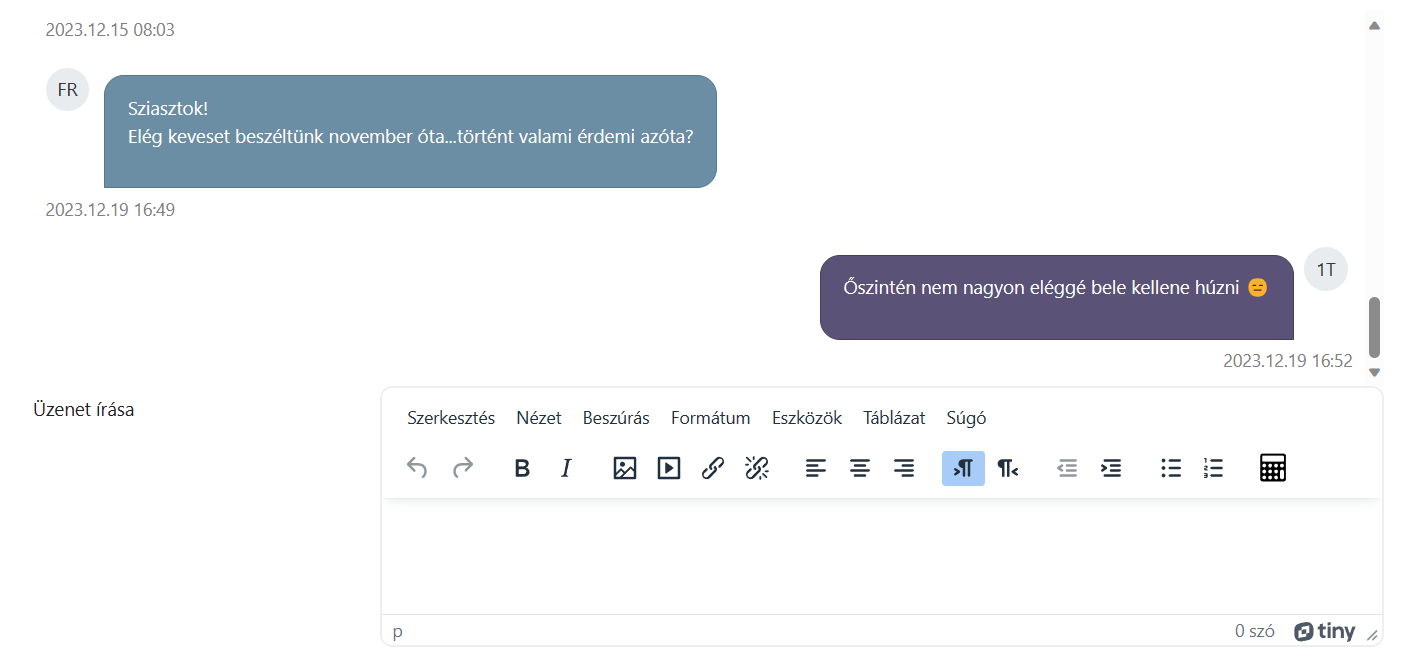
\includegraphics[width=0.8\textwidth, frame]{images/uzenet.png}
	\caption{Beszélgetés a csoporton belül}
\end{figure}

\subsection{Feladat leadása}

Ha a csoport elkészült a feladatával, lehetősége van az arra kijelölt személynek feltölteni a megoldást a \textit{Leadott feladatok} menüpontban. Egy feladatot többször is le lehet adnia a csoportnak, de mindig a legfrissebb leadás fog megjelenni az értékelő tanároknak. A feladat leadására a Moodle fájlkezelője áll rendelkezésre, így már a portálra korábban feltöltött fájlok között is tudnak a felhasználók böngészni. A feladat feltöltési korláta a rendszerben és PHP-ban beállított feltöltési korlátnak felel meg. A hallgatónak csak egy fájlfeltöltésre van lehetősége, viszont az állomány típusa nem számít, így tömörített állományt is elfogad az alkalmazás. Feladatot egészen a beadási határidőig tölthet fel a csapat, ez a határidő minden menüpontban megjelenik a hallgatók számára a modulon belül. A leadott feladatok biztonsági mentésnél is elmentésre kerülnek.
\begin{figure}[H]
	\centering
	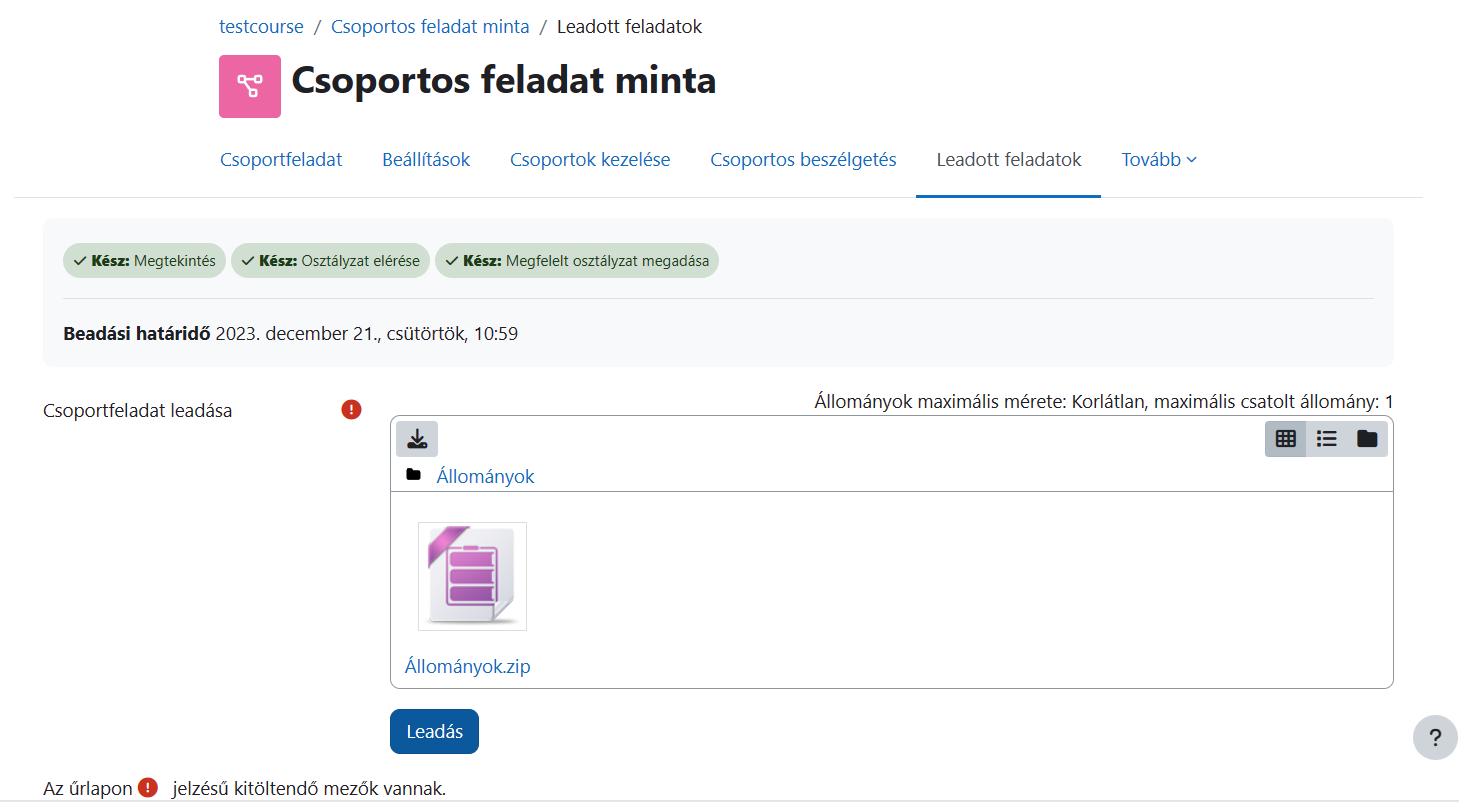
\includegraphics[width=0.8\textwidth, frame]{images/feladat.png}
	\caption{Feladat leadási felület}
\end{figure}

\subsection{Egyéb oldalak}

A hallgatóknak lehetőségük van bizonyos oldalak korlátozott elérésére. Ha megfelelő szerepkörrel rendelkeznek a csoporton belül, akkor van lehetőségük új csoport létrehozására. Saját csoportjuk adatainak módosítására is kaphatnak jogosultságot, így tudják növelni manuálisan a csoportlétszámot, ha több tagra van szükségük. Emellett van lehetőségünk saját csoportjukhoz új tagokat felvenni a navigációs menün keresztül. A feladat leadása is szerepkör jogosultsághoz kötött. Ha szeretnénk, hogy minden csoporttag leadhassa a feladatot, akkor az \textit{Engedélyek} menüponton keresztül hozzá kell adnunk a Hallgatót a \textit{Csoport feladat leadása} engedélyhez. A felhasználó jogosultságától függően a modul navigációs sávjában megjelenhetnek új menüpontok, amik a felhasználót az általa elérhető oldalra navigál tovább. Ha a felhasználó olyan oldalt szeretne elérni, amihez nem rendelkezik a szükséges jogosultsággal, akkor egy általános hibaüzenetet (Jogosultság megtagadva) kap a felületen.

\begin{figure}[H]
	\centering
	\subcaptionbox{Navigációs menü jogosultság nélkül}{
		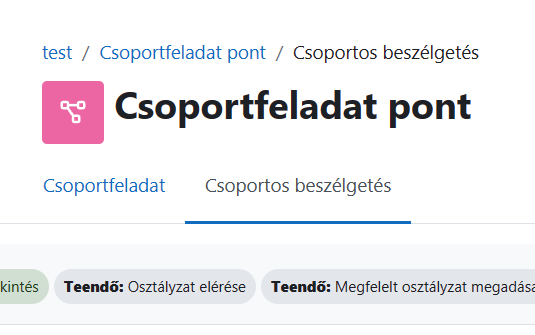
\includegraphics[width=0.35\linewidth,frame]{images/navigacio_ures.png}}
	\hspace{5pt}
	\subcaptionbox{Navigációs menü az összes jogosultsággal}{
		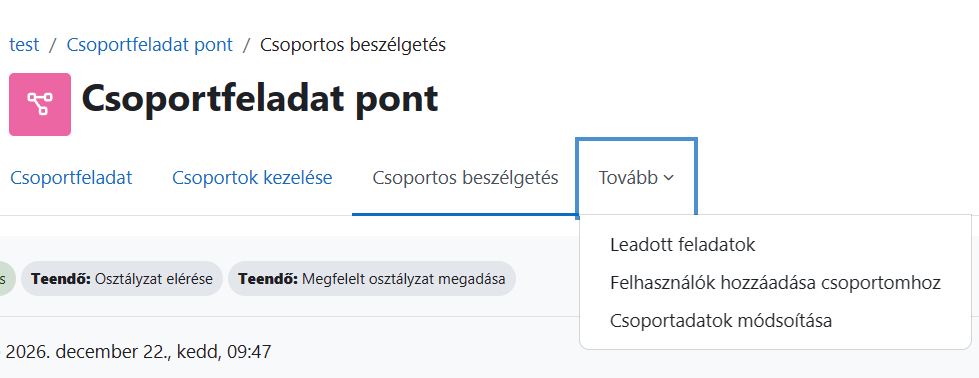
\includegraphics[width=0.55\linewidth,frame]{images/navigacio_teljes.png}}
	\caption{Navigációs menü dinamikus megjelenése}
	\label{fig:example-2}
\end{figure}
\cleardoublepage

\chapter{Fejlesztői dokumentáció}
\label{ch:impl}

\section{Fejlesztés célja}

A Moodle számos felhasználói igényt lefed a kurzusain belül, viszont a csoportos munkamegosztás szervezésére a rendszernek nincs konkrét dobozos megoldása. Különböző tevékenységmodulok működései támogatják például a csoportos feladatleadást, vagy egy fórumon belüli kommunikációt, viszont ezen tevékenységek egymástól függetlenül működnek és nincs lehetőségünk a funkciók összekötésére. A fejlesztés célja egy egyedi tevékenységmodul létrehozása, mely képes a csoportok kezelésére, feladatok kiosztására, illetve a csoporttagok közötti kommunikáció megvalósítására. Emellett a feladat leadása, majd értékelése is a modul részét fogja képezni. 

A Moodle számos tevékenységmodullal operál, melyek segédprogramként kerültek megvalósításra, így új fejlesztése a Moodle által biztosított API-n keresztül történhet meg. Fontos, hogy az új segédprogram fejlesztése megfeleljen a Moodle fejlesztési szabványainak, így későbbi Moodle verziókban sem lesz nehéz integrálni a segédprogramot. A tevékenységmodulokkal szemben állított elvárásoknak meg kell felelnie az alkalmazásnak, így a fejlesztés során számos feladat elve adott, ezeken kívül szükséges a személyes fejlesztési célok megvalósítása és egy hosszútávon támogatható segédprogram fejlesztése.

\section{Megvalósítási terv}

Lényeges, hogy a modul harmonizáljon a keretrendszer által kínált összképpel és a felhasználói élménnyel. Ehhez felhasználjuk a megfelelő renderereket és objektumokat, hogy létrehozzuk a különböző felületi elemeket.

A "Csoportfeladat" egy tevékenységmodul. A Moodle-ben rendszerint ezt a kurzuskezelő felületen keresztül lehet létrehozni és konfigurálni. A tevékenységmodulok létrehozásakor a tanároknak meg kell adniuk a következő információkat:
\begin{compactitem}
    \item A tevékenység neve: ez a név megjelenik a kurzusban, és a tanulók ezt használhatják a tevékenység megtalálásához.
    \item A tevékenység leírása: ez a leírás segíti a tanulókat a tevékenység megértésében.
    \item A tevékenység beállításai: ezek a beállítások szabályozzák a tevékenység működését.
\end{compactitem}
A beállítások szabályozhatják a értékelés módját, a feladat határidejét és a teljesítmény értékelésének módját.
Ezen nézetek felületi megjelenése adott, így a tevékenységmodulon belüli nézetekről lesz fontos a drótvázterveket és sablonokat előkészíteni.

\subsection{Drótváztervek}

A modul nézeteinek tervezése során fontos, hogy a felületi elemek illeszkedjenek a Moodle arculatába. Ezért törekedni kell a minimális egyedi CSS és minél több beépített felületi elem használatára. A drótvázak a tevékenységmodul által generált környezet tartalmának bemutatására szolgálnak, így a rendszer által generált menüpontok és egyéb felületi elemek nem kerültek modellezésre. A drótváztervek Justinmind\footnote{\url{https://www.justinmind.com/}} segítségével készültek el.

\subsubsection{Csoportok listázása}

\begin{figure}[H]
	\centering
	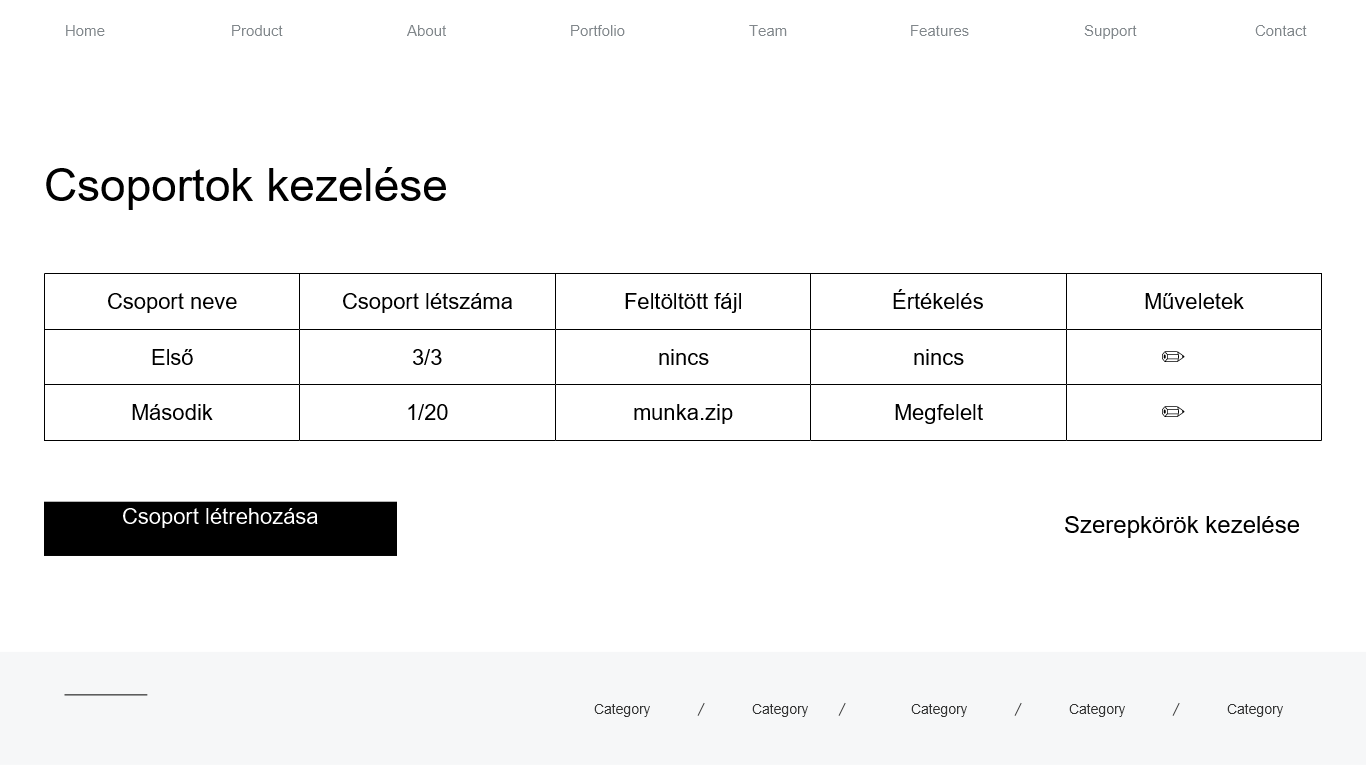
\includegraphics[width=0.8\textwidth]{images/csoportok_kezelese_wire.png}
	\caption{Csoportok kezelése drótvázterv}
\end{figure}
\textbf{Oldal funkciói} :

\begin{compactitem}
	\item Meglévő csoportok listázása táblázatban. Szükséges oszlopok és adatok megjelenítése.
        \begin{compactitem}
            \item Csoport nevének megjelenítése
            \item Csoport jelenlegi létszámának és maximális létszámának megjelenítése (például 5/10 formátumban)
            \item Csoport által leadott feladatmegoldás letöltési linkjének megjelenítése
            \item Csoport értékelésének kiírása
            \item Csoport műveleteinek megjelenítése
        \end{compactitem}
        \item Új csoport hozzáadása oldal elérése
        \item Szerepkörök kezelése oldal elérése
        \item Meglévő csoport adatainak módosítása (fogaskerék ikon)
        \item Meglévő csoport törlése (kuka ikon)
        \item Csoporthoz felhasználók hozzáadása (ember ikon)
        \item Csoport értékelése (ceruza ikon)
 \end{compactitem}

\subsubsection{Csoport létrehozása és módosítása}

\begin{figure}[H]
	\centering
	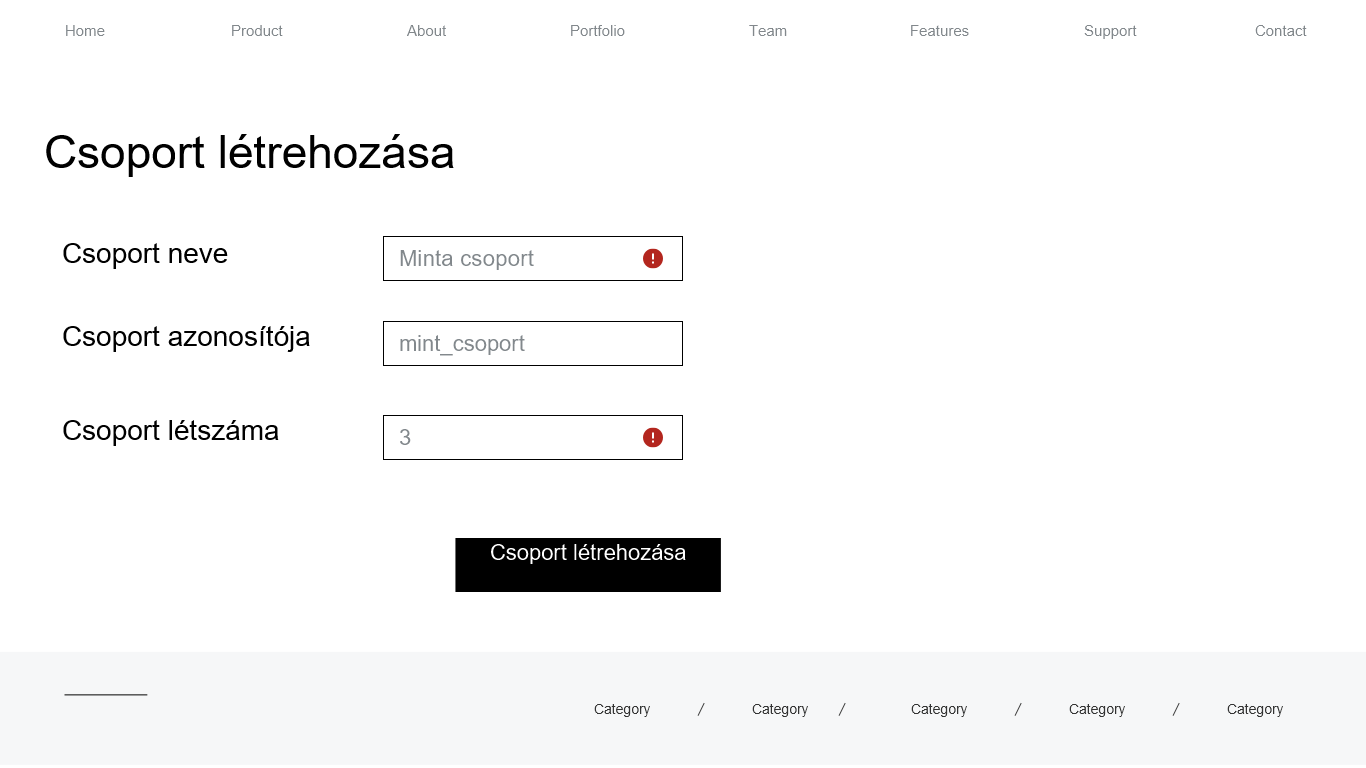
\includegraphics[width=0.8\textwidth]{images/csoport_letrehozasa_wire.png}
	\caption{Csoport létrehozása drótvázterv}
\end{figure}

\textbf{Oldal funkciói} :

\begin{compactitem}
	\item  Csoport nevének, azonosítójának és méretének felvétele és validálása
        \item Új csoport esetén, gombnyomásra adatok alapján új rekord létrehozása
        \item Létező csoport esetén, gombnyomásra adatok alapján meglévő rekord frissítése
 \end{compactitem}

\subsubsection{Csoport értékelése}

\begin{figure}[H]
	\centering
	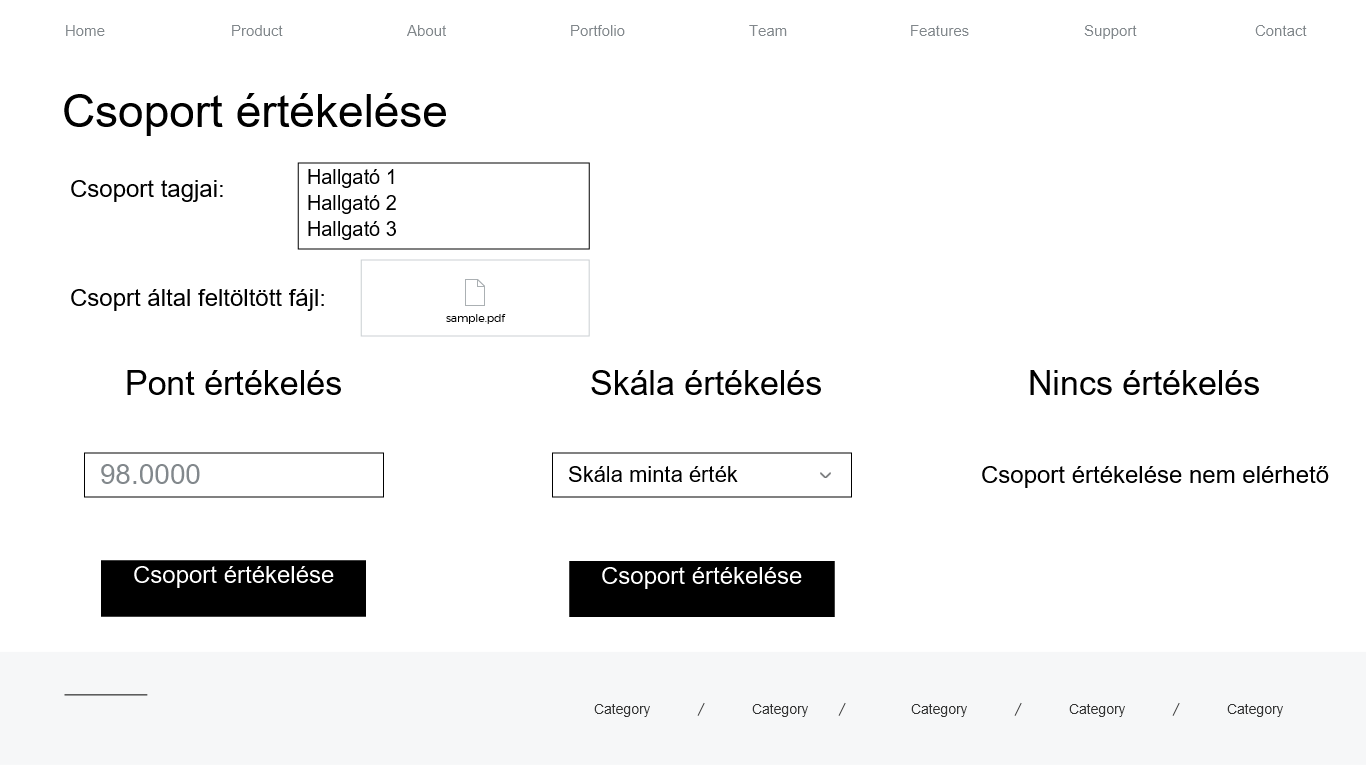
\includegraphics[width=0.8\textwidth]{images/csoport_ertekelese_wire.png}
	\caption{Csoport értékelése drótvázterv}
\end{figure}

\textbf{Oldal funkciói} :

\begin{compactitem}
	\item Modulon belül beállított pontozási módszer helyes megjelenítése:
            \begin{compactitem}
                \item Pontozási módszer esetén számbevitel mező megjelenítése
                \item Skálázási módszer esetén a skála értékeinek megjelenítése a mezőben
                \item Ha nincs módszer beállítva, ne jelenjen meg semmi
            \end{compactitem}
        \item Értékelés megadása után csoportok listázásánál jelenjen meg az eredmény
        \item Minden csoporttag számára kerüljön az eredmény rögzítésre az erre fenntartott pontozási riportban (kurzus szinten)
 \end{compactitem}

\subsubsection{Csoporthoz felhasználók hozzáadása}

\begin{figure}[H]
	\centering
	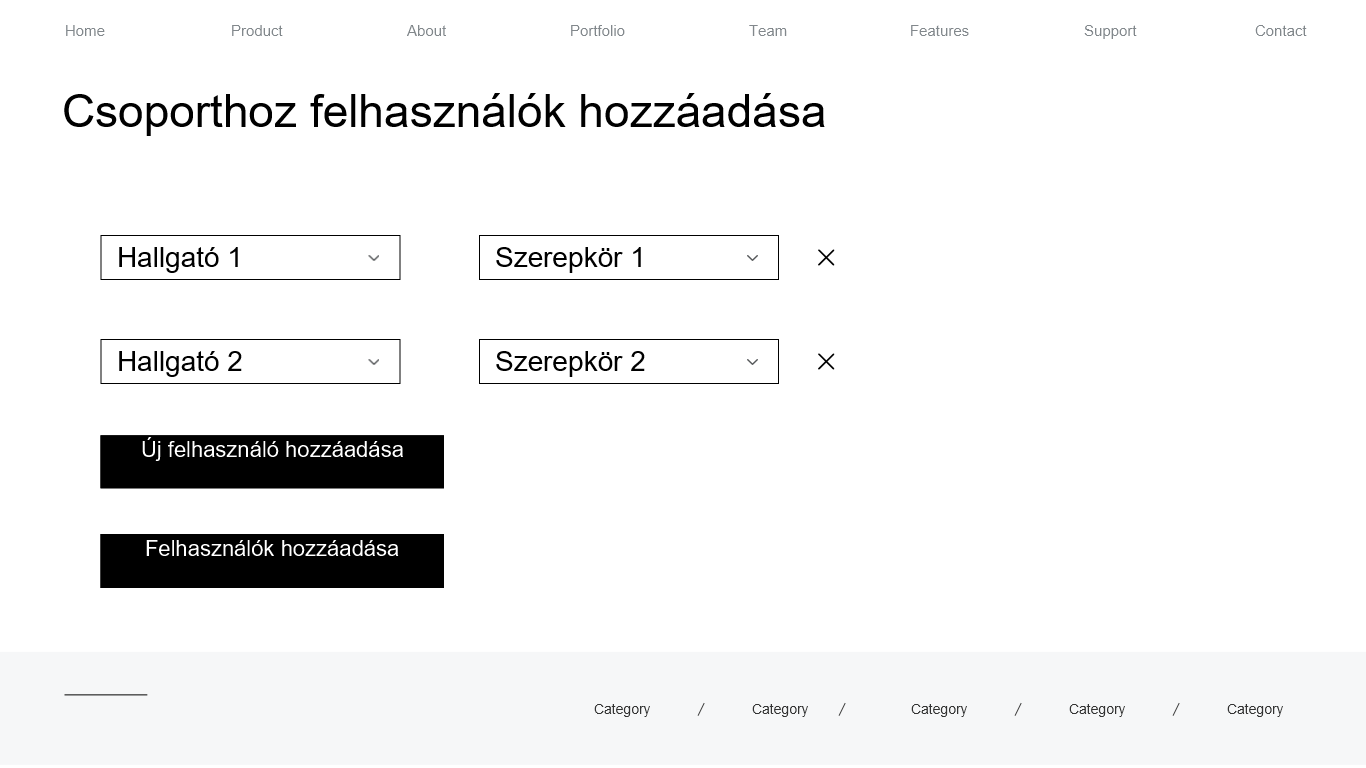
\includegraphics[width=0.8\textwidth]{images/felhasznalok_hozzaadasa_wire.png}
	\caption{Csoporthoz felhasználók hozzáadása drótvázterv}
\end{figure}

\textbf{Oldal funkciói} :

\begin{compactitem}
	\item Jelenlegi csoporttagok megjelenítése a megfelelő szerepekkel a nevük mellett
    \item Maximum annyi felhasználót tudjon az oldalt kezelő személy hozzáadni a csoporthoz, amennyi a csoport beállításainál definiálésra került.
    \item Egy felhasználót nem lehet kétszer hozzáadni
    \item Más csoportok tagjai ne jelenjenek meg a lehetséges felhasználók között
    \item A kurzusba beíratott felhasználók jelenjenek meg a lehetséges felhasználók között
    \item A felhasználókhoz lehet szerepkört rendelni, de ez nem kötelező
    \item Űrlap leadása után a felhasználók a megfelelő szerepkörökkel a legyenek a csoport tagjai
    \item Ha egy felhasználót töröltünk a csoportból, már ne legyen a csoport része
    \
 \end{compactitem}

\subsubsection{Szerepkörök listázása}

\begin{figure}[H]
	\centering
	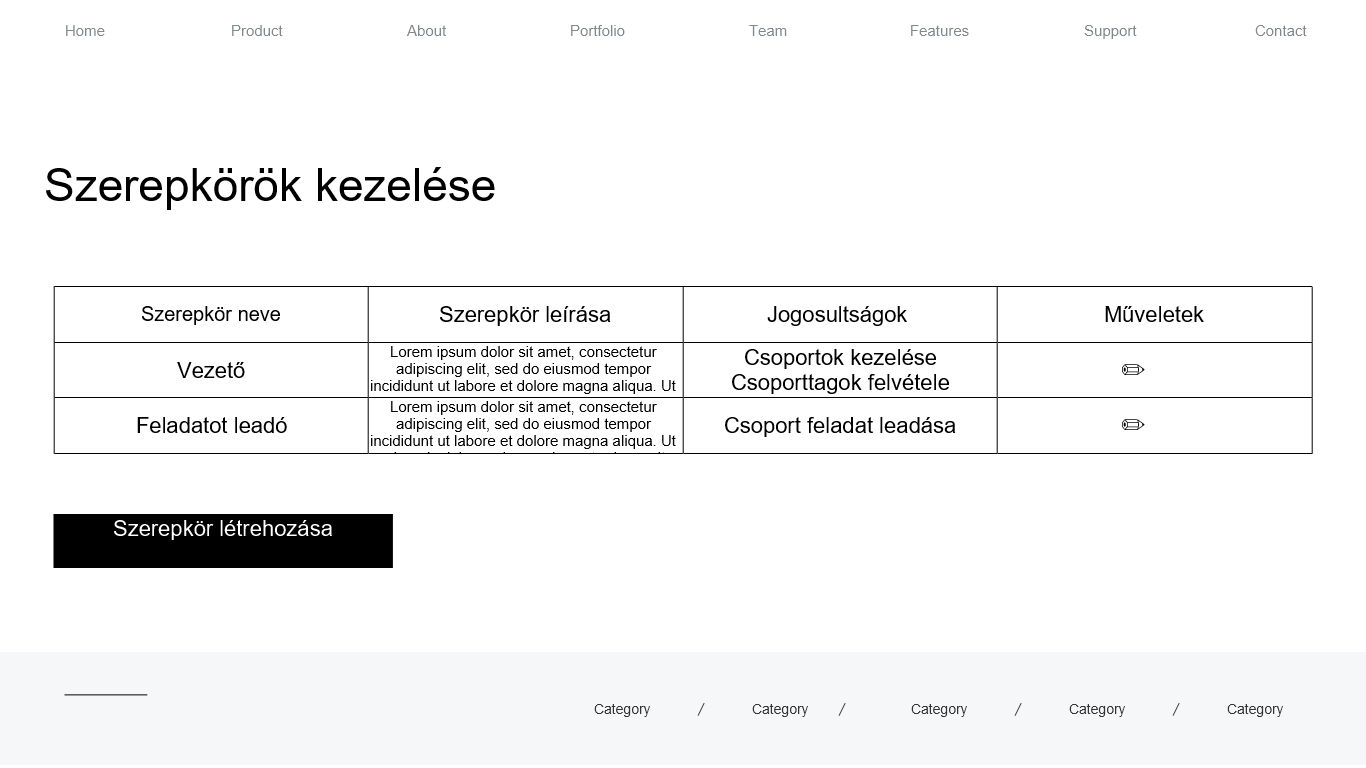
\includegraphics[width=0.8\textwidth]{images/szerepkorok_kezelese_wire.png}
	\caption{Szerepkörök kezelése drótvázterv}
\end{figure}
\textbf{Oldal funkciói} :

\begin{compactitem}
	\item Meglévő szerepkörök listázása táblázatban. Szükséges oszlopok és adatok megjelenítése.
        \begin{compactitem}
            \item Szerepkör nevének megjelenítése
            \item Szerepkör leírásának megjelnítése (HTML adat)
            \item Szerepkör jogosultságainak megtekintése
            \item Szerepkör műveleteinek megjelenítése
        \end{compactitem}
        \item Új Szerepkör hozzáadása oldal elérése
        \item Meglévő Szerepkör adatainak módosítása (fogaskerék ikon)
        \item Meglévő Szerepkör törlése (kuka ikon)
 \end{compactitem}

\subsubsection{Szerepkörök létrehozása és módosítása}

\begin{figure}[H]
	\centering
	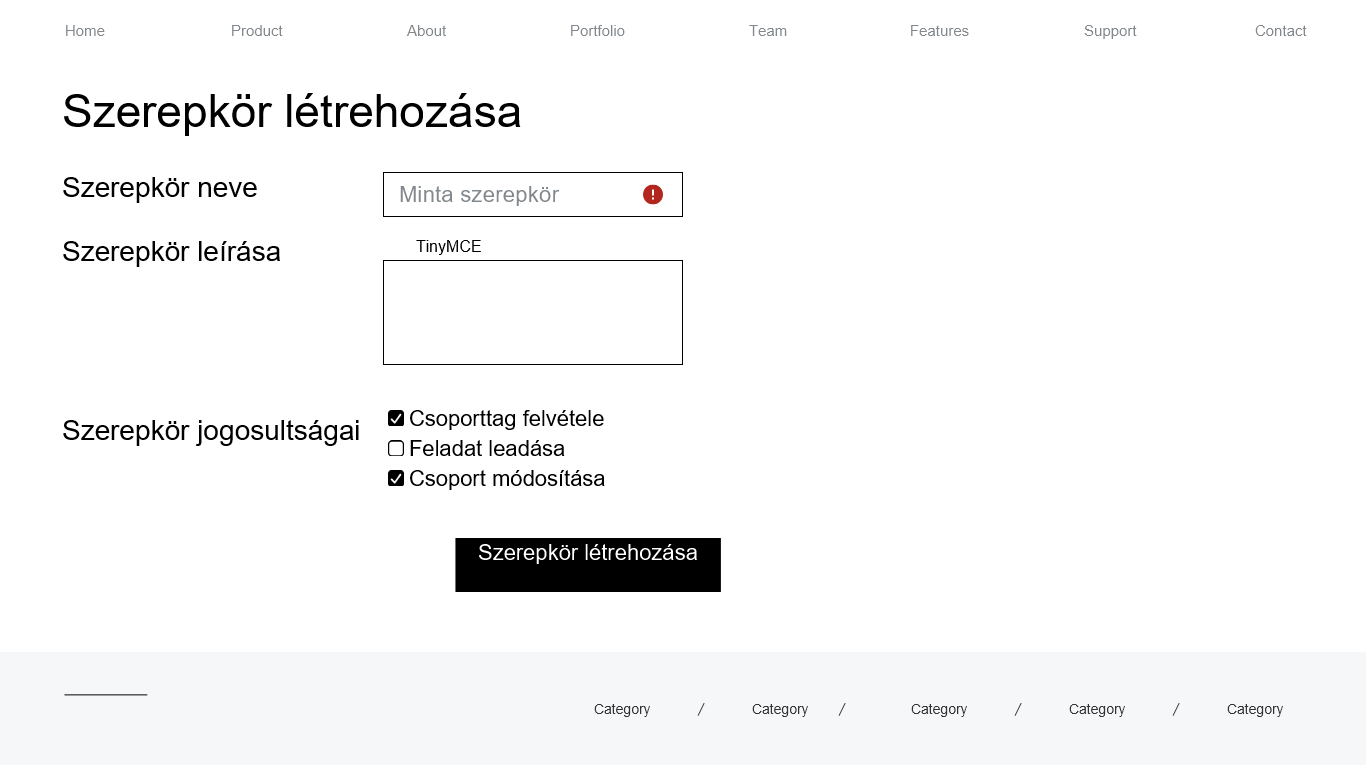
\includegraphics[width=0.8\textwidth]{images/szerepkor_letrehozasa_wire.png}
	\caption{Szerepkör létrehozása drótvázterv}
\end{figure}
\textbf{Oldal funkciói} :

\begin{compactitem}
	\item  Szerepkör nevének, leírásának és jogosultságainak felvétele és validálása
         \item Felvehető jogosultságok megjelenítése
        \item Új szerepkör esetén, gombnyomásra adatok alapján új rekord létrehozása
        \item Létező szerepkör esetén, gombnyomásra adatok alapján meglévő rekord frissítése
 \end{compactitem}

\subsubsection{Feladat leadása}

\begin{figure}[H]
	\centering
	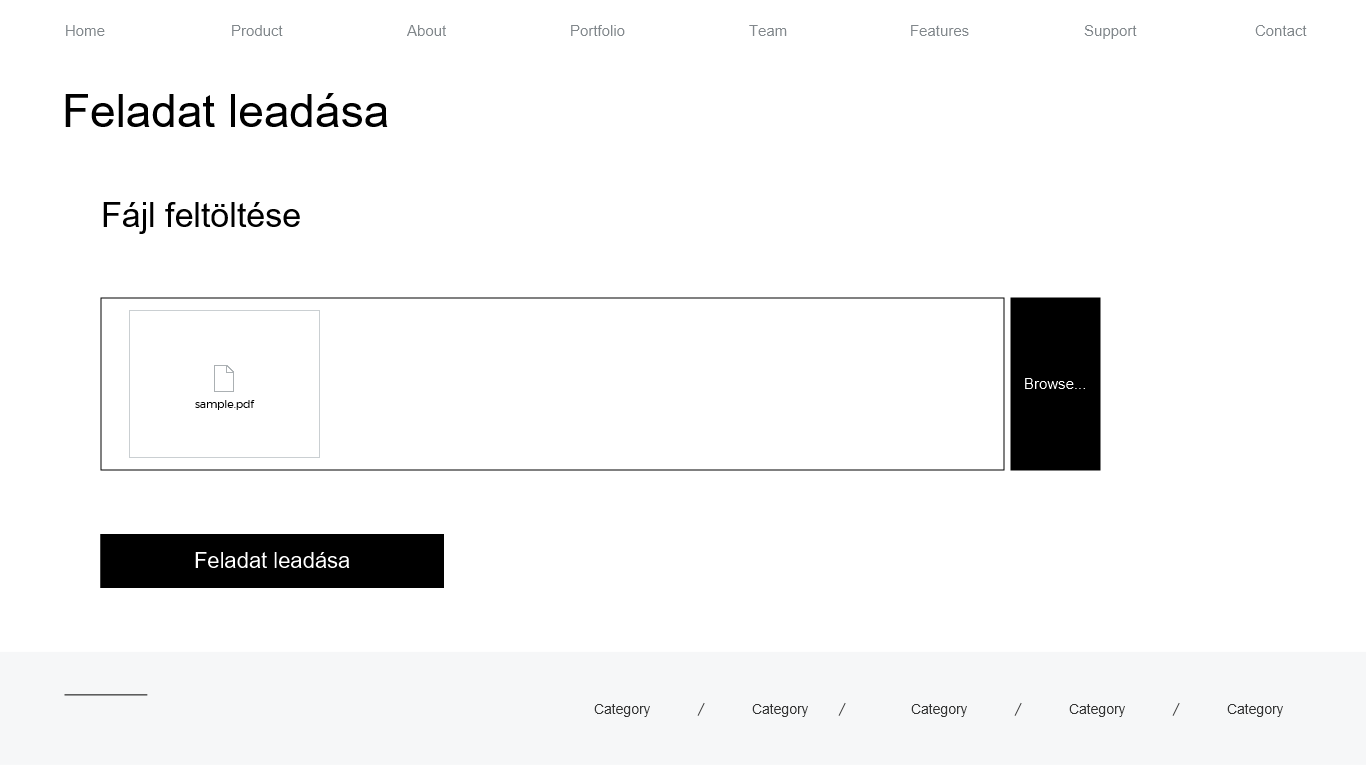
\includegraphics[width=0.8\textwidth]{images/feladat_leadasa_wire.png}
	\caption{Feladat leadása drótvázterv}
\end{figure}

\textbf{Oldal funkciói} :

\begin{compactitem}
	\item A beadási határidő ellenőrzése és oldalon lévő űrlap zárolása, ha a hallgató kifutott a feltöltési határidőből
         \item Leadott fájl feltöltésének érzékelése, helyes feltöltés esetén felhasználó számára visszajelzés küldése
 \end{compactitem}

\subsubsection{Csoportos beszélgetés}

\begin{figure}[H]
	\centering
	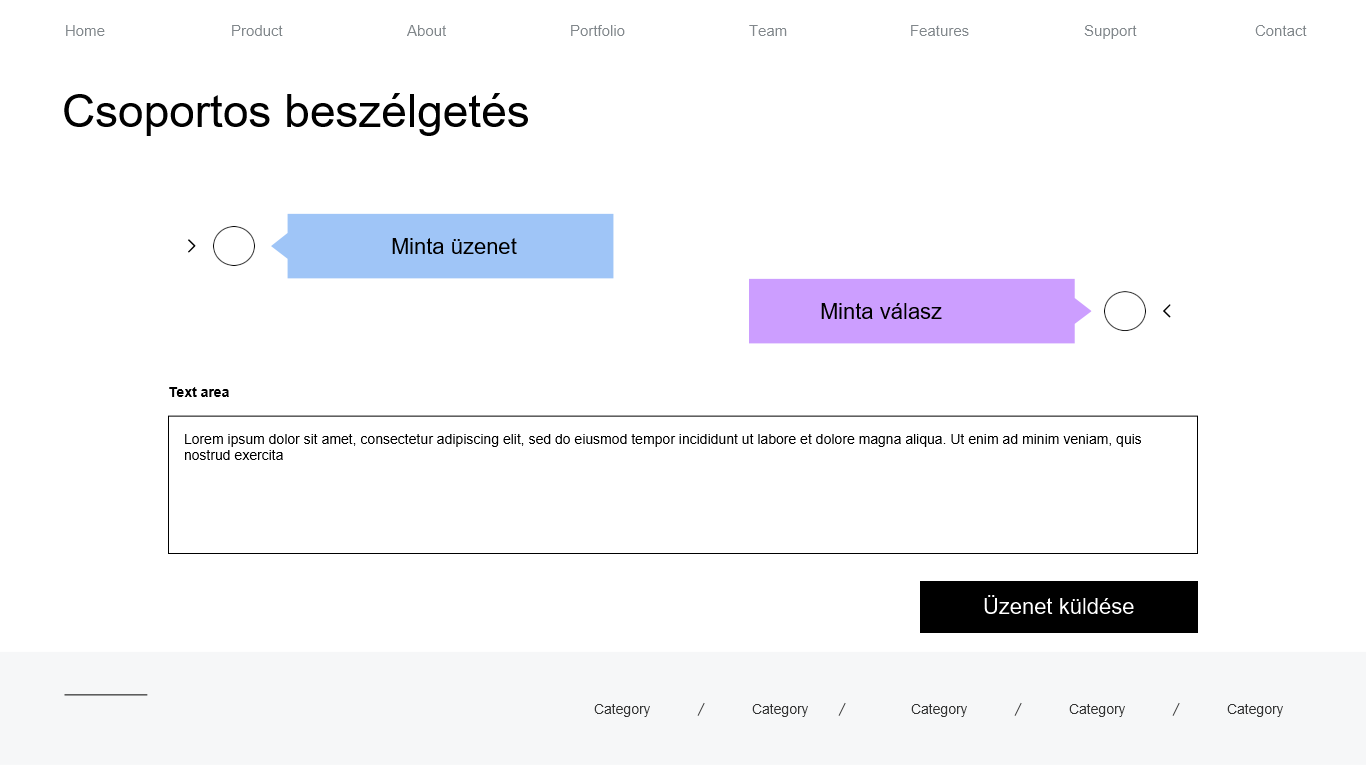
\includegraphics[width=0.8\textwidth]{images/csoportos_beszelgetes_wire.png}
	\caption{Csoportos beszélgetés drótvázterv}
\end{figure}

\textbf{Oldal funkciói} :

\begin{compactitem}
	\item  A hallgató számára az eddigi üzenetek időrendben való megjelenítése
    \item A hallgató új üzenetet írhat az erre a célra fenntartott szerkesztőben
    \item Üzenet küldése esetén jelenjen meg a felhasználó számára az új üzenete a beszélgetési panelben
    \item Ha egy másik felhasználó küldött üzenetet a rendszerben, rövidesen jelenjen meg üzenete a hallgató beszélgetési paneljében
 \end{compactitem}

\section{Adatbázis felépítése}

A modul adattábláinak felhasználása a Moodle konvencióival összhangban van, és az ezeknek megfelelő relációs adatbázis struktúrát alkalmazza. A rendszer a Moodle által már tárolt adatokra és az ezeket tartalmazó táblákra épül. Az adattábla kapcsolatok a \ref{fig:example-1} ábrán találhatóak. A Moodle által használt prefix a \textit{mdl}, még a segédprogram által használt prefix a \textit{groupproject}, így könnyebben átlátható, a segédprogram által létrehozott táblák halmaza.

\begin{figure}[H]
	\centering{
		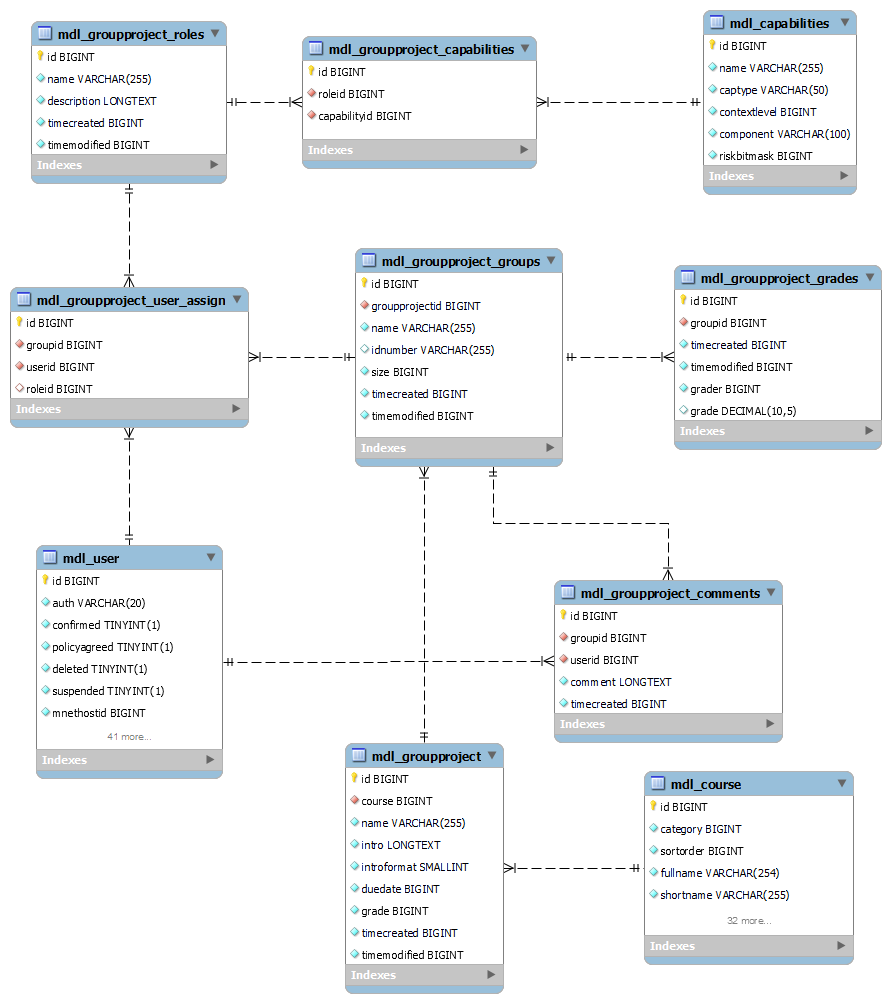
\includegraphics[width=0.9\linewidth]{images/tabla_modell.png}}
	\caption{Adattábla kapcsolatok}
	\label{fig:example-1}
\end{figure}
Az ábrán nincsenek felültetve a Moodle által kezelt, viszont a kapcsolatok szempontjából nehezen modellezhető kapcsolatok. Ilyen típusú kapcsolatok és adatok tárolásáról, bővebben az  \ref{adat:egyeb-1} címsorban lesz szó.

\subsection{Adattáblák}

\subsubsection{\textbf{Mdl\_groupproject: Kurzuson belüli tevékenységmodul instancia táblája}}
\begin{compactitem}
	\item id (BIGINT(10), NOT NULL, AUTO\_INCREMENT): egyedi azonosító
    \item course (BIGINT(10), NOT NULL, DEFAULT 0): kurzus azonosítója
    \item name (VARCHAR(255), NOT NULL): tevékenység neve
    \item intro (LONGTEXT, NOT NULL): tevékenység leírása
    \item introformat (INT(4), NOT NULL, DEFAULT 0): tevékenység leírásának típusa
     \item duedate (BIGINT(10), NOT NULL, DEFAULT 0): beadás határideje
    \item grade (BIGINT(10), NOT NULL, DEFAULT 0): tevékenység pontozása
    \item timecreated (BIGINT(10), NOT NULL, DEFAULT 0): tevékenység létrehozás dátuma
    \item timemodified (BIGINT(10), NOT NULL, DEFAULT 0): tevékenység módosításának dátuma
 \end{compactitem}

\subsubsection{\textbf{Mdl\_groupproject\_groups: Tevékenységen belüli csoportok adatai}}
\begin{compactitem}
	\item id (BIGINT(10), NOT NULL, AUTO\_INCREMENT): egyedi azonosító
    \item groupprojectid (BIGINT(10), NOT NULL, DEFAULT 0): tevékenységmodul azonosítója
    \item name (VARCHAR(255), NOT NULL): csoport neve
    \item idnumber (VARCHAR(255),  NULL, DEFAULT NULL): csoport azonosítója
    \item size (BIGINT(10), NOT NULL, DEFAULT 0): csoport mérete
    \item timecreated (BIGINT(10), NOT NULL, DEFAULT 0): csoport létrehozás dátuma
    \item timemodified (BIGINT(10), NOT NULL, DEFAULT 0): csoport módosításának dátuma
 \end{compactitem} 

\subsubsection{ \textbf{Mdl\_groupproject\_roles: Modul által kezel szerepkörök adatai}}
\begin{compactitem}
	\item id (BIGINT(10), NOT NULL, AUTO\_INCREMENT): egyedi azonosító
    \item name (VARCHAR(255), NOT NULL): szerepkör neve
    \item description (LONGTEXT, NOT  NULL): szerepkör leírása
    \item timecreated (BIGINT(10), NOT NULL, DEFAULT 0): szerepkör létrehozásának dátuma
    \item timemodified (BIGINT(10), NOT NULL, DEFAULT 0): szerepkör módosításának dátuma
 \end{compactitem} 

\subsubsection{  \textbf{Mdl\_groupproject\_user\_assign: Felhasználó csoporthozzárendelések adatai}}
\begin{compactitem}
	\item id (BIGINT(10), NOT NULL, AUTO\_INCREMENT): egyedi azonosító
    \item groupid (BIGINT(10), NOT NULL): csoport azonosítója
    \item userid (BIGINT(10), NOT NULL): felhasználó azonosítója
    \item roleid (BIGINT(10),  NULL): szerepkör azonosítója
 \end{compactitem} 

\subsubsection{{\textbf{Mdl\_groupproject\_comments: Felhasználó csoportbejegyzések adatai}}}
\begin{compactitem}
	\item id (BIGINT(10), NOT NULL, AUTO\_INCREMENT): egyedi azonosító
    \item groupid (BIGINT(10), NOT NULL): csoport azonosítója
    \item userid (BIGINT(10), NOT NULL): felhasználó azonosítója
    \item comment (LONGTEXT, NOT NULL): bejegyzés tartalma
    \item timecreated (BIGINT(10), NOT NULL, DEFAULT 0): bejegyzés létrehozásának dátuma
 \end{compactitem} 

\subsubsection{ {\textbf{Mdl\_groupproject\_grades: Csoporteredmények adatai}}}
\begin{compactitem}
	\item id (BIGINT(10), NOT NULL, AUTO\_INCREMENT): egyedi azonosító
    \item groupid (BIGINT(10), NOT NULL, DEFAULT 0): csoport azonosítója
    \item grader (BIGINT(10), NOT NULL, DEFAULT 0): értékelő tanár azonosítója
    \item grade (BIGINT(10), NOT NULL, DEFAULT 0): érdemjegy
    \item timecreated (BIGINT(10), NOT NULL, DEFAULT 0): eredmény létrehozásának dátuma
    \item timemodified (BIGINT(10), NOT NULL, DEFAULT 0): eredmény módosításának dátuma
 \end{compactitem} 

\subsubsection{  {\textbf{Mdl\_groupproject\_grades: Szerepkör jogosultság hozzárendelések}}}
\begin{compactitem}
	\item id (BIGINT(10), NOT NULL, AUTO\_INCREMENT): egyedi azonosító
    \item roleid (BIGINT(10), NOT NULL, DEFAULT 0): szerepkör azonosítója
    \item capabilityid (BIGINT(10), NOT NULL, DEFAULT 0): jogosultság azonosítója
 \end{compactitem} 

\subsection{Egyéb adattáblák} \label{adat:egyeb-1}

\subsubsection{{\textbf{Mdl\_modules: Elérhető tevékenységmodulok adatai}}}
 
A rendszerbe telepített elérhető tevékenység modulok tárolására szolgáló tábla. Telepítésnél egy rekord jön létre az egyedi modulunknak, a modul nevével és alapértelmezett láthatóságával. Az itt meghatározott azonosítóra fog hivatkozni a kurzuson belüli \textit{course\_modules} tábla.

\subsubsection{{\textbf{Mdl\_course\_modules: Kurzuson belüli tevékenységmodulok adatai}}}
 
Kurzuson belül új tevékenységmodul létrehozásánál két táblába kerülnek az új rekord adatai. A rendszerszinten kezelt \textit{course\_modules} tábla a kurzus számára releváns információkat tartalmazza. A \textit{module} és \textit{instance} oszlopok segítségével képes meghatározni a párhuzamosan létrejött instancia tábla nevét és az abba tárolt instancia rekordot, amit a segédprogramunk esetben már a \textit{groupproject} tábla tartalmaz.

\subsubsection{{\textbf{Mdl\_grade\_items: Pontozási tételek táblája}}}
 
Kurzus és tevékenység esetén pontozási tételeket hozhatunk létre a kurzus kontextusában. Ha a tételünk egy tevékenységre hivatkozik az \textit{itemtype}, \textit{itemmodule} és az \textit{iteminstance} oszlop segítségével funkcionálisan meghatározhatjuk a megfelelő instancia táblát és annak rekordját.

\subsubsection{{\textbf{Mdl\_files: Portálszinten tárolt fájlok adatai}}}
 
A fájlok kezelésére a Moodle egy úgynevezett File System API\footnote{\url{https://docs.moodle.org/dev/File_System_API}}-t használ. A Moodle File Storage API a fájl tartalmának checksum\footnote{Checksum: Ellenőrző összeg, adatátvitel vagy adattárolás hibátlanságának ellenőrzését segítő módszer.} (Moodle-ben \textit{ContentHash}-ként hivatkoznak rá) generálásával deduplikációt hajt végre. A tárolt fájlokat komponensekhez és fájlterületekhez rendelhetjük egy tételazonosító segítségével. Ezekre az adatokra rendre a \textit{component}, \textit{filearea} és \textit{itemid} oszlopok hivatkoznak, így ezen adatok mentén tudjuk a File API-n keresztül lekérni a szükséges fájlt. A segédprogramunk esetén a csoportok által leadott fájlok kapcsolódnak ehhez a táblához. A leadott fájlokat a \textit{mod\_groupproject} komponensen belül (ez részben adott), tároljuk, a \textit{groupproject\_submission} fájlterületen. Az itt tárolt fájlok tételazonosítói, a csoportok azonosítóira hivatkoznak, így minden csoportnak meg tudjuk határozni a beadott munkáját.

\subsection{Engedélyek}

A segédprogram által definiált engedélyek és azok alapértelmezett szerepköreinek táblázata.

\begin{table}[H]
	\centering
	\begin{tabular}{ | m{0.2\textwidth} | m{0.2\textwidth} | m{0.3\textwidth} | m{0.15\textwidth} | }
		\hline
		\textbf{Engedély azonosítója} & \textbf{Engedély neve} & \textbf{Alapértelmezett szerepkörök} & \textbf{Csoporttag számára elérhető?}  \\  
		\hline \hline
		\emph groupproject: view & Csoportfeladat tevékenység megtekintése & Minden felhasználó & Nem \\
		\hline
		\emph groupproject: addinstance &  Csoportfeladat tevékenység létrehozása & Tanár, Igazgató & Nem \\
		\hline
		\emph groupproject: post\_comment & Csoportmeg-jegyzés írása & Nem szerkesztő tanár, Tanár, Igazgató & Nem \\
		\hline
        \emph groupproject: managegroup & Csoport kezelése & Nem szerkesztő tanár, Tanár, Igazgató & Igen \\
		\hline  
        \emph groupproject: creategroup & Csoport létrehozása & Nem szerkesztő tanár, Tanár, Igazgató & Igen \\
		\hline  
        \emph groupproject: modifygroup & Csoport módosítása & Nem szerkesztő tanár, Tanár, Igazgató & Igen \\
		\hline  
        \emph groupproject: deletegroup & Csoport törlése & Nem szerkesztő tanár, Tanár, Igazgató & Nem \\
		\hline  
        \emph groupproject: adduser & Csoporthoz felhasználók hozzáadása & Nem szerkesztő tanár, Tanár, Igazgató & Igen \\
		\hline  
        \emph groupproject: gradegroup & Csoport értékelése & Nem szerkesztő tanár, Tanár, Igazgató & Nem \\
		\hline  
        \emph groupproject: submitfile & Csoport feladat leadása & Nem szerkesztő tanár, Tanár, Igazgató & Igen \\
		\hline  
	\end{tabular}
	\caption{Egyedi engedélyek táblázata}
	\label{tab:example-1}
\end{table}
A fent említett engedélyek telepítésnél a \textit{capibilities} táblába kerülnek, az \textit{access.php} fájl adatai alapján.

\section{Architekturális terv}
A Moodle-ben a modulok olyan önálló, önállóan telepíthető és futtatható kiegészítők, amelyek új funkciókat vagy szolgáltatásokat adnak a rendszerhez. A modulok számos különböző kategóriába sorolhatók, például:

\begin{compactitem}
    \item Tevékenység modul: ezek a modulok új funkciókat adnak a kurzusokhoz, például feladatokat, teszteket, wikiket vagy fórumokat.
    \item Adminisztrációs modulok: ezek a modulok új funkciókat adnak az adminisztrátorok számára, például felhasználói fiókok kezelését, jelentések készítését vagy biztonsági beállításokat.
    \item Rendszermodulok: ezek a modulok a Moodle alaprendszerének működését érintik, például a teljesítményt, a biztonságot vagy a nyelvi támogatást.
\end{compactitem}

\subsection{Fájl szerkezet}

A rendszerben a modulok fájljai a Moodle telepítési helyén találhatók. A fájlszerkezet a következőképpen néz ki:

/moodle/[modul\_típusa]/[modul\_név]/[modul\_fájlok]

A Csoportfeladat fájljai a \textit{mod} mappában találhatók. A név egyedi azonosítóként szolgálnak, amelyek az elérési útvonalra utalnak, például jelen esetben a  \textit{mod\_groupproject}. A modulok fájljai általában a következő típusú fájlokat tartalmazzák:
\begin{compactitem}
    \item Sablonok: a sablonok a modulok felhasználói felületét határozzák meg.
    \item Kiegészítők: a kiegészítők a modulok funkcionalitását bővítik.
    \item Konfigurációs és rendszer által előírt fájlok: az adatbázis sémák a modulok adatbázisaiban tárolt adatok struktúráját határozzák meg, illetve a modul rendszerbe való integrálást segítik elő.
    \item Egyéb fájlok: Minden egyéb osztálynak, template-nek és Javascript fájlnak, tesztesetnek megvan a rendszer által javasolt helye. Az egyéb modul működését elősegítő fájlokat így egy szabvány mentén tudjuk rendszerezni.
\end{compactitem}
A modulok fájlszerkezetének részletei a modul típusától függően változhatnak. Ezeknek az általános szabályoknak a figyelembevételével került implementálásra a program.

\subsection{Az egyes fájlok, mappák leírásai:}
\begin{compactitem}
    \item \textbf{version.php}: Minden modul esetén szükséges egy version.php fájl, hiszen ez tartalmazza az aktuális verziószámot és ennek a módosítása teszi lehetővé a rendszer által is érzékelhető verziófrissítést. Emellett ez a fájl tartalmazza azt is, hogy milyen más modul szükséges a telepítéshez. 
    \item \textbf{lib.php}: Általános függvények kerülnek ide, melyeket általában a keretrendszer hív meg. Ilyenek például a modul által támogatott funkciók listája, a modul saját navigációs sávja, a fájlküldést segítő műveletek, illetve tevékenységmodul esetén az instancia tábla karbantartása a kurzusmodul által generált adatok segítségével. 
    \item \textbf{locallib.php}: A segédprogram saját függvénykönyvtára, mely nem szükséges a Moodle-el való kommunikációhoz. A Csoportfeladat esetében itt kerültek kiszervezésre a megjelenítésért felelős scriptek törzsének kirajzolását támogató függvényei.
    \item \textbf{externallib.php}: A webszolgáltatások végpontjainak függvénydefiníciói. Szükséges minden végpont bemenő és kimenő paramétereinek pontos definiálása, illetve a tényleges függvény megírása, ami lefut a végpont meghívásakor. Az alkalmazás a szinkron kommunikáció közben próbálja majd elérni ezeket a végpontokat és az innen kapott adatok alapján rajzolja ki dinamikusan az üzeneteket a hallgatóknak.
    \item \textbf{settings.php}: A globális beállításokat tartalmazó fájl, illetve a beállításoknak a navigációs sávjának manipulálása.
    \item \textbf{db mappa}:
    \begin{compactitem}
        \item \textbf{install.xml}: A telepítéskor létrehozandó adatbázis táblákat tartalmazza a fájl.
        \item \textbf{access.php}: Azokat a jogosultságokat definiálja, amelyek a modul használatához szükségesek.
        \item \textbf{upgrade.php}: A modul verzióemelésénél lefutó PHP script, új adatok és adattáblák manipulálására használható. Az alkalmazásnál szükséges volt utólag módosítani néhány oszlop nevét és működését, így ezek visszavezetésre kerültek az install.xml-be is.
        \item \textbf{log.php}: Az alkalmazás használata közben keletkezett logokat tudjuk itt definiálni egy tömbbe.
        \item \textbf{services.php}: A webszolgáltatásokat tartalmazó PHP script. A hallgatók csoportos beszélgetése közben szükséges, hogy a modul frontend része tudjon adatokat küldeni és kérni a szervertől.
    \end{compactitem}
    \item \textbf{lang mappa}: A modul nyelvi fájljait tartalmazó mappa. Angol fordítás kötelező, ezeket a nyelvi elemeket az en mappában tároljuk. Egyéb fordítás esetén (például magyar), új mappát kell létrehozni (hu), és ugyan azzal a fájl elnevezéssel létrehozni a kívánt nyelvi fordítással elkészített lang fájlt.
    \item \textbf{amd mappa}: A JavaScript forrás fájlok az src mappában találhatóak. Ezeket a Moodle a Grunt\footnote{Grunt: JavaScript feladatfuttató, \url{https://gruntjs.com/}} segítségével készíti elő a build mappába a megfelelő kódanalízis (ESLint\footnote{ESLint: Statikus Javascript kódelemző, \url{https://eslint.org/}} segítségével) és optimalizáció után. A segédprogramunk esetén a beszélgetés paneljében található üzenetek kezelése lett ide kiszervezve, JQuery\footnote{JQuery: Javascript keretrendszer , \url{https://jquery.com/}} segítségével.
    \item \textbf{templates mappa}: A segédprogram által használt sablonok mappája. A Moodle által hivatalon támogatott websablon rendszer a Mustache template\footnote{Mustache template: Logika nélküli websablonrendszer,  \url{https://mustache.github.io/}}. A Csoportfeladat esetén a beszélgetési panel kezdeti állapota Mustache template segítségével készült.
    \item \textbf{pix mappa}: A modul ikonját tartalmazó mappa.
    \item \textbf{backup mappa}: A modul biztonsági mentését és annak visszatöltését kezelő osztályokat tartalmazó mappa. Mivel a Csoportfeladat Moodle 4.2-ben lett fejlesztve, így már csak a \textit{moodle2} által definiált biztonsági mentési protokollokat támogatja.
    \item \textbf{classes mappa}: Az osztálydefiníciókat tartalmazza.
    \begin{compactitem}
        \item \textbf{event mappa}: A használat során keletkezett események osztályai találhatóak meg itt.
        \item \textbf{output mappa}: A különböző felületi elemek reprezentálására szolgáló osztályok mappája.
        \item \textbf{local mappa}: A segédprogram nem rendszer által használt osztályainak tárolására szolgáló mappa.
    \end{compactitem}
    \item \textbf{tests mappa}: A PHPUnit\footnote{PHPUnit: PHP egységtesztelő keretrendszer, \url{https://phpunit.de/}} és Behat\footnote{Behat: PHP eseményvezérelt tesztkeretrendszer, \url{https://docs.behat.org/}} teszteket tartalmazó mappa.
    \item \textbf{egyéb PHP fájlok a gyökérkönyvtárban}: Minden egyéb PHP fájl a modulon belül egy elérhető oldalnak felel meg. (például \textit{group.php} = Csoportok kezelése oldal). Ezek a PHP scriptek az oldal paramétereit és header/footer kirajzolását segítik elő az adott kontextus segítségével. Az oldal tartalmát (lényegében a body-t) a script a \textit{locallib}-be defininált függvények segítségével rajzolja ki.
\end{compactitem}


\subsection{Osztályok}

A segédprogramon belül van lehetőségünk egyedi osztályokat létrehozni. Ezek lehetnek teljesen egyedi, általunk definiált osztályokból leszármaztatott osztályok , de van lehetőségünk meglévő, a rendszer által definiált osztályokból is származtatni azokat. Az osztályainkat, általában a \textit{classes} mappába definiáljuk, így a fejlesztés során én is ezt a konvenciót követtem. Az UML-ek StarUML\footnote{\url{https://staruml.io/}} segítségével készültek el.

\subsubsection{Felületi megjelenésért felelő osztályok}

Az \textit{output} mappán belül található osztálydefiníciók, mind a felületi megjelenésért felelő objektumok tárolására szolgálnak. Az itt megírt osztálydefiníciók meglévő Moodle osztályokból kerültek származtatásra, és táblázatok és űrlapok megjelenését segítik. Ezek az osztályok felületi elemek validálását és megjelenítését segítik elő. 
\begin{figure}[H]
	\centering{
		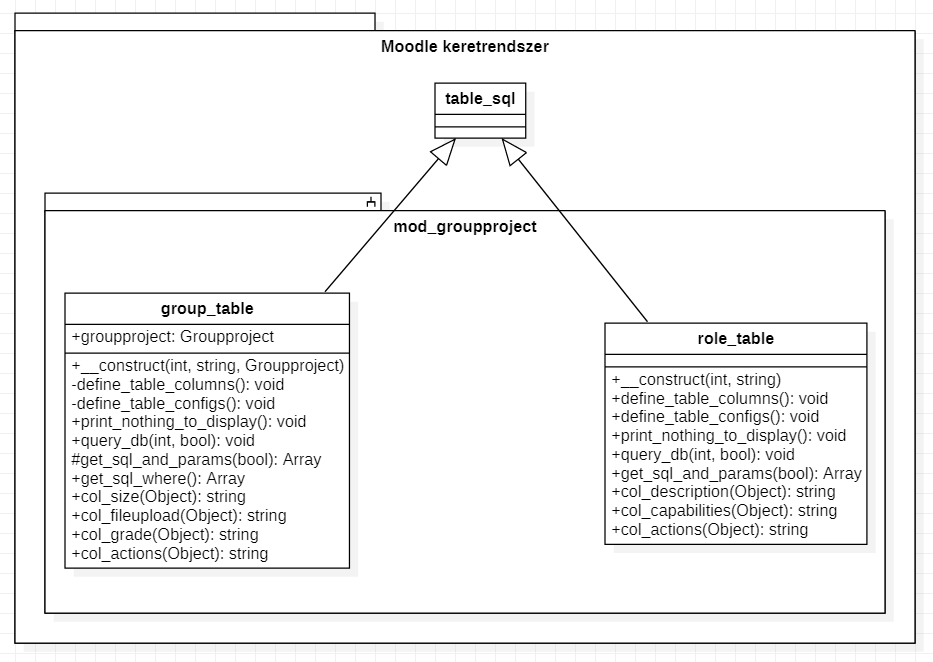
\includegraphics[width=0.9\linewidth]{images/table_sql.png}}
	\caption{Táblázat osztálydefiníciók}
\end{figure}

\begin{figure}[H]
	\centering{
		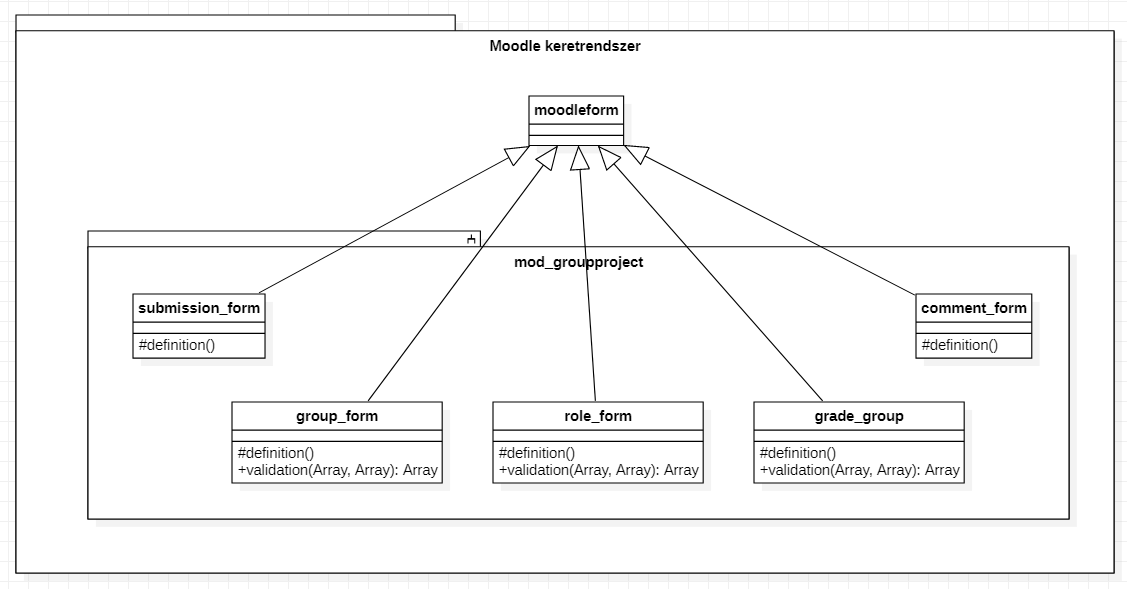
\includegraphics[width=0.9\linewidth]{images/moodleform.png}}
	\caption{Űrlap osztálydefiníciók}
\end{figure}
\subsubsection{Rendszerintegrációért felelős osztályok}

A megfelelő rendszerintegráció érdekében a segédprogramunk különböző pontjain van lehetőségünk fix Moodle osztályokból származtatni saját megoldásainkat. Ezek az osztályok valamilyen Moodle által támogatott funkció absztrakt megfelelői, melyeket minden rendszerbe integrált segédprogramnak van lehetősége megvalósítani. A leszármaztatás után a segédprogram támogatni fogja az érintett funkciót.

A \textit{mod\_groupproject} az alábbi ilyen megoldásokat tartalmazza:
\begin{compactitem}
    \item \textbf{Backup}: Biztonsági mentésért felelős interfész. Biztonsági mentés végrehajtásának lépéseit és a mentett XML\footnote{XML: Extensible Markup Language, általános célú leírónyelv} tartalmának visszatöltésének lépéseit tartalmazzák az ezért felelős osztályok a segédprogramban. 
    \item \textbf{Event}: Moodle események kiváltásáért felelős osztályok halmaza. Jelen esetben a tevékenységmodul megtekintésénél váltjuk ki, így tudunk különböző teljesítési beállításokat használni a modulban.
    \item \textbf{Dates}: A tevékenység fontosabb dátumainak reprezentálásáért felelős osztály. A beadási határidőt itt tudjuk a tevékenységmodulon kívüli felületen jelezni a hallgatók számára. 
    \item \textbf{External\_Api}: Moodle webszolgáltatások támogatására fenntartott osztály. A Moodle REST\footnote{REST: Representational State Transfer, reprezentációs állapotátvitel} és SOAP\footnote{SOAP: Simple Object Access Protocol, távoli eljáráshívás-protokoll } protokollt támogat, ám ezek számára az üzenetek struktúráját és tartalmát egy absztrakt API osztály kezeli. A segédprogramunk esetében, mi a beszélgetés funkció AJAX\footnote{AJAX: Asynchronous JavaScript and XML, interaktív webalkalmazások létrehozására szolgáló webfejlesztési technika} hívásainál használjuk az osztály adta lehetőségeket.
    \item \textbf{Modform}: A tevékenységmodulunk létrehozásáért felelős osztály. Az itt található űrlapmodell azért felelős, hogy tudjuk manipulálni, a tevékenység létrehozásánál kötelezően megjelenítendő mezőket. Ilyen extra mezők például a pontozási beállítások, vagy a beadási határidő kitöltése.
\end{compactitem}

\begin{figure}[H]
	\centering{
		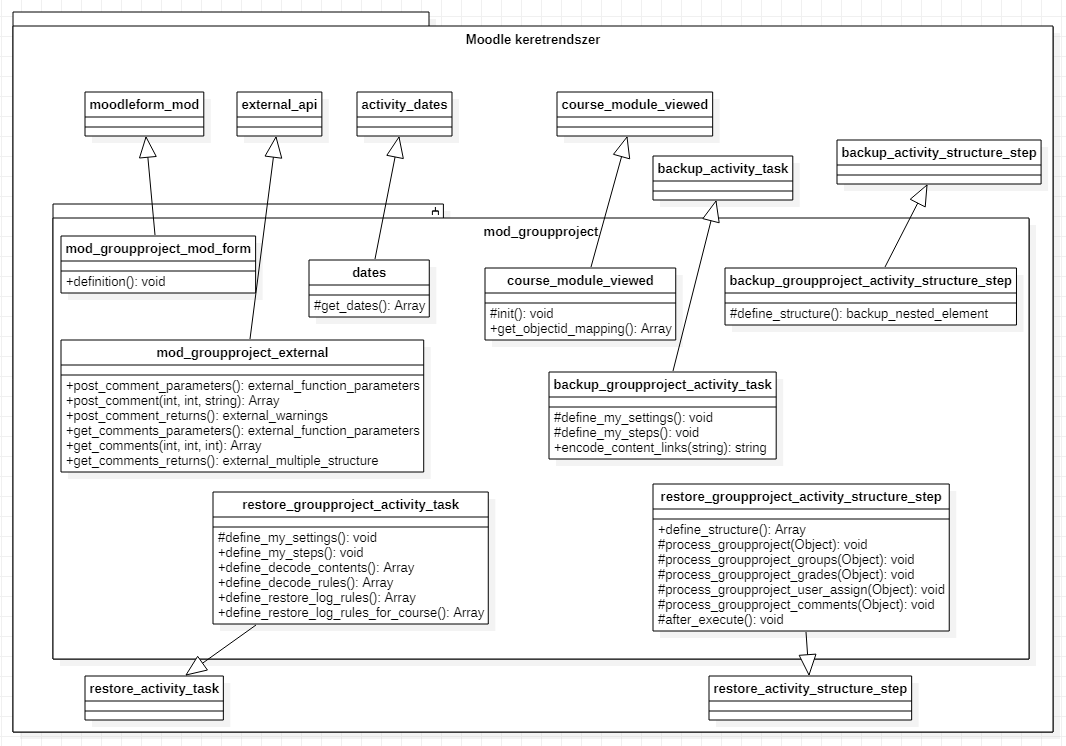
\includegraphics[width=0.9\linewidth]{images/system_uml.png}}
	\caption{Rendszerintegrációért felelős osztálydefiníciók}
\end{figure}

\subsubsection{Tevékenységmodul osztályok}

A modul helyes működése érdekében saját osztályai is vannak a segédprogramnak, melyek pusztán az adatbáziskommunikáció elősegítését, illetve az adatok izolációját segítik elő a mindennapi működésben. 

\begin{compactitem}
    \item \textbf{Entitások}: Az adatbázis kommunikáció elősegítése érdekében bevezetésre került egy \textit{entity} ősosztály, melynek minden leszármazottja, egy a segédprogram által létrehozott adattáblára hivatkozik. Az ebből leszármazott osztályok a CRUD\footnote{CRUD: Create, Read, Update, and Delete, perzinsztens tárolásra szolgáló operációk} folyamatokon kívül számos a modul működését elősegítő metódussal rendelkeznek.

\begin{figure}[H]
	\centering{
		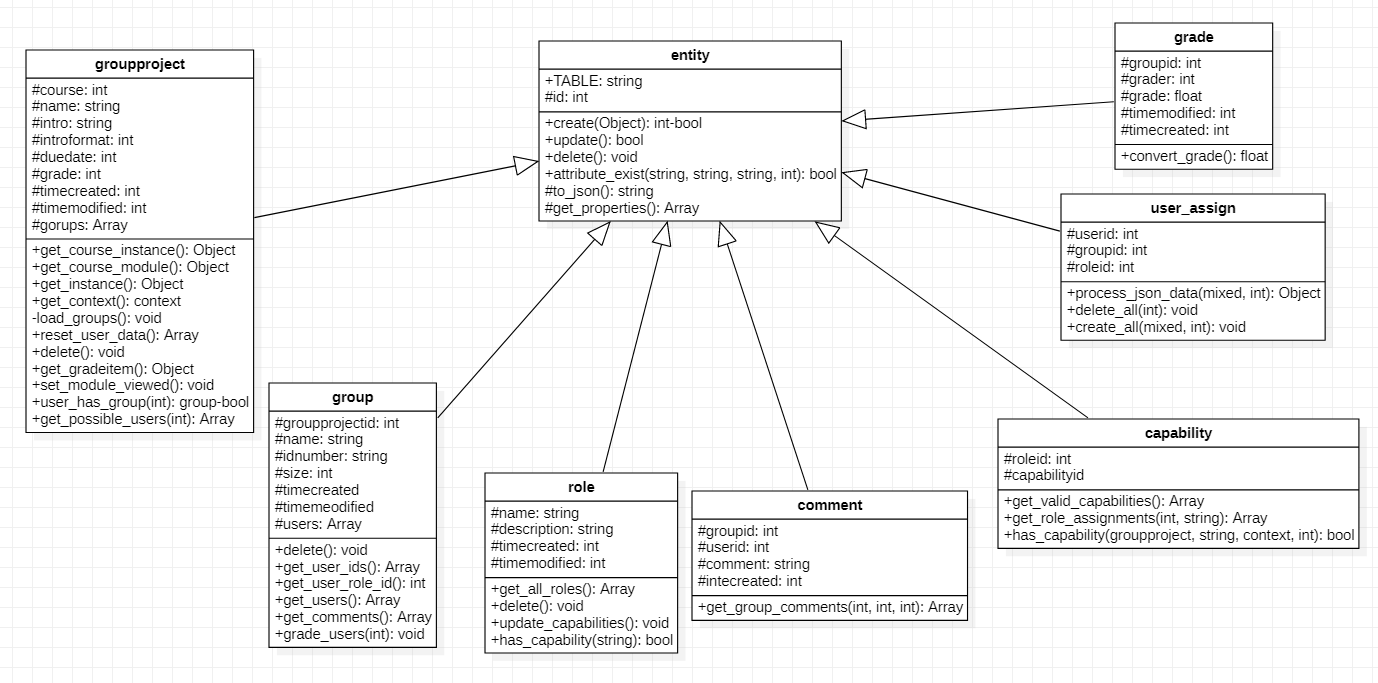
\includegraphics[width=0.9\linewidth]{images/entity.png}}
	\caption{Entitás osztályok}
\end{figure}
    
    \item \textbf{Factory osztály}: Az entitások létrehozását segítő Factory osztály. Képes \textit{stdClass}-ok segítségével meghívni a különböző osztályok konstruktorait, így az adatbázisból kiolvasott rekordokat könnyen tudja egy sokkal komplexebb objektummá konvertálni.
    \item \textbf{Loader osztály}: Sok esetben a különböző PHP scriptek egymásnak csak egyszerű változókat tudnak átadni az URL-eken keresztül, így egy azonosító alapján kell egy teljes objektumot létrehozni. Ezek betöltésére szolgál a \textit{loader} osztály, melyik képes egy azonosító alapján bármely entitást betölteni.
    \item \textbf{Generátor osztályok}: A Mustache template és JQuery által használt nézetek, egy előre megadott struktúrájú adathalmazra támaszkodnak. Ezek előállításában segít a \textit{generator} osztály, mely a nézetek számára releváns adatokat rendszerezi.
\end{compactitem}

\section{Tesztelési terv}

A Moodle támogatja az egység-, illetve az eseményvezérelt tesztelést. A modul teszteseteit a test mappába lehet megírni. Támogatottak a PHPUnit által használt konvenciók, illetve a Behat Gherkin\footnote{Gherkin: Viselkedésellenőrző nyelv \url{https://cucumber.io/docs/gherkin/}} nyelven írt tesztesetei. Az egységtesztek kipróbálásához szükséges elvégezni a szükséges környezeti beállításokat. A beállítás lépéseit rendszerünk alábbi linkjén érhetjük el: \url{/admin/tool/phpunit/index.php}  Az egységtesztelés saját táblákkal dolgozik, így ezeknek egy egyedi prefix-et kell adnunk, hogy el tudja különíteni a rendszer a tesztelés céljából fenntartott táblákat, illetve a rendszer által használt táblákat.

\subsection{PHPUnit tesztesetek}

Az egységtesztek célja, hogy a modul által kezelt osztályok metódusait validálja és azok működésének sajátosságait minél jobban lefedje. A fejlesztés során számos kisebb forráskódbeli módosításnál sikerült hibákat kiszűrni a Unit tesztek segítségével. Ahol indokolt volt, tesztvezérelt fejlesztési metódusok kerültek alkalmazásra a fejlesztés közben, így számos osztály viselkedésének megírása tesztesetekkel lett alátámasztva.

Az alábbi programkomponensek egységtesztelése került implementálásra:

\begin{compactitem}
\item \textbf{Tevékenységmodul tesztesetei:}
\begin{compactitem}
    \item Tevékenységmodul entitás létrehozása, módosítása és törlése
    \item Tevékenységmodul csoportjainak betöltése
    \item Felhasználó csoporttagság ellenőrzése tevékenységmodul kontextusában.
\end{compactitem}
\item \textbf{Csoportok tesztesetei:}
\begin{compactitem}
    \item Csoport létrehozása, módosítása
    \item Csoport törlése és az ezzel kapcsolatos csoportadatok törlése
    \item Csoport tagjainak lekérése
    \item Csoport adott felhasználójának szerepének lekérdezése
    \item Csoport tagjainak azonosítójának lekérdezése
\end{compactitem}
\item \textbf{Felhasználói hozzárendelések tesztesetei:}
\begin{compactitem}
        \item Felhasználói hozzárendelés létrehozása, módosítása és törlése
\end{compactitem}
\item \textbf{Szerepkörök tesztesetei:}
\begin{compactitem}
        \item Szerepkör létrehozása és módosítása
        \item Szerepkör törlése és a szerepkörhozzárendelések törlésének ellenőrzése
        \item Szerepkör jogosultságok létrehozása (Jogosultság teszteseteivel részben összefügg)
        \item Szerepkör jogosultság ellenőrzése
\end{compactitem}
\item \textbf{Jogosultság tesztesetei:}
\begin{compactitem}
        \item Jogosultság létrehozása, módosítása és törlése
        \item Szerepkör jogosultságainak lekérdezése
        \item Felhasználó rendelkezik-e az adott jogosultsággal egy adott tevékenységmodulon belül?
\end{compactitem}
\item \textbf{Üzenet tesztesetei:}
\begin{compactitem}
        \item Üzenet létrehozása, módosítása és törlése
\end{compactitem}
\item \textbf{Eredmény tesztesetei:}
\begin{compactitem}
        \item Eredmény létrehozása, módosítása és törlése
        \item Eredmény értékének konvertálása felhasználó számára
\end{compactitem}
\item \textbf{Factory osztály tesztesetei}:
\begin{compactitem}
        \item Tevékenységmodul létrehozása \textit{stdClass} alapján
        \item Csoport létrehozása \textit{stdClass} alapján
        \item Felhasználói hozzárendelés létrehozása \textit{stdClass} alapján
        \item Szerepkör létrehozása \textit{stdClass} alapján
        \item Jogosultság létrehozása \textit{stdClass} alapján
        \item Üzenet létrehozása \textit{stdClass} alapján
        \item Eredmény létrehozása \textit{stdClass} alapján
\end{compactitem}
\item \textbf{Loader osztály tesztesetei}:
\begin{compactitem}
        \item Tevékenységmodul létrehozása azonosító segítségével
        \item Csoport létrehozása azonosító segítségével
        \item Felhasználói hozzárendelés létrehozása azonosító segítségével
        \item Szerepkör létrehozása azonosító segítségével
        \item Jogosultság létrehozása azonosító segítségével
        \item Üzenet létrehozása azonosító segítségével
        \item Eredmény létrehozása azonosító segítségével
\end{compactitem}
\end{compactitem}

\subsection{Behat tesztesetek}

Az eseményvezérelt tesztek segítségével valós programhasználatot tudunk modellezni. A keretrendszer által használt Gherkin nyelv könnyen olvasható és a struktúrája is egyszerű, lényegében feltételek mentén utasításokat fogalmazunk meg a gép számára. A Moodle-ben kialakított Behat keretrendszer is a segédprogramok támogatására szolgál. Az alaprendszer már számos általános utasítás definícióját és tesztesetét tartalmazza, így alkalmazásunknak elég a saját komponenseire fókuszálnia.

Az alábbi programkomponensek eseményvezérelt tesztelése került implementálásra:

\begin{compactitem}
    \item \textbf{Csoport létrehozása és módosítása űrlap:}
    \begin{compactitem}
        \item Üres űrlap esetén hibát jelez a rendszer
        \item Helytelen csoportlétszám esetén hibát dob a rendszer
        \item Név és csoportlétszám megadás, illetve az űrlap leadása után a rendszer elnavigál minket egy másik oldalra
    \end{compactitem}
    \item \textbf{Szerepkör létrehozása és módosítása űrlap:}
    \begin{compactitem}
        \item Üres űrlap esetén hibát dob a rendszer
        \item Név megadása, illetve az űrlap leadása után a rendszer elnavigál minket egy másik oldalra
    \end{compactitem}
    \item \textbf{Csoportok listázása oldal megtekintése :}
    \begin{compactitem}
        \item Ha nincs csoport nem jelenik meg a táblázat
        \item Ha a tevékenységmodulon belül létezik csoport megjelenik a táblázat
        \item Ha a csoport létrehozása gombra kattintunk a rendszer elnavigál minket egy másik oldalra
        \item Ha a Szerepkörök kezelése linkre kattintunk a rendszer elnavigál minket egy másik oldalra
        \item A csoportok táblázat \textit{Műveletek} oszlopban található ikonok közül mindegyik kattintható 
    \end{compactitem}
    \item \textbf{Szerepkörök listázása oldal megtekintése :}
    \begin{compactitem}
        \item Ha nincs szerepkör nem jelenik meg a táblázat
        \item Ha létezik szerepkör megjelenik a táblázat
        \item Ha a szerepkör létrehozása gombra kattintunk a rendszer elnavigál minket egy másik oldalra
        \item A szerepkörök táblázat \textit{Műveletek} oszlopban található ikonok közül mindegyik kattintható 
    \end{compactitem}
\end{compactitem}

\section{Továbbfejlesztési lehetőségek}

\begin{compactitem}
 \item Különböző feladatbeadási lehetőségek biztosítása (például esszé szöveges formátumban vagy egyszerre több fájlleadás). Ezeket a lehetőségeket bővítmény (subplugin) szinten is meg lehet valósítani.
\item Dinamikus mezők támogatása csoportok és szerepkörök esetén, így extra információkat tudunk felvenni vagy kérni a csoporttagoktól.
\item  Moodle szinten kezelt csoporttokkal (cohort) és szerepkörökkel (role) való integráció.
\item Naptárbejegyzések készítse a rendszeren belül, ha adtunk meg beadási határidőt.
	\item Automatikus értesítők a hallgatók számára a beadási határidő lejárta előtt. Az értesítő tárgyának és szövegének módosítása különböző kontextusokban. 
\item Fájl előnézet funkció bizonyos állománytípusok esetén (például PDF vagy PNG állománytípusok megjelenítése).
\item Bővebb tesztesetek.
\item Moodle 4.3 és PHP8.3 támogatása
\item Bővebb naplózási esetek. Felhasználó komment írásnál, fájlfeltöltésnél, és osztályozásnál esemény kiváltása.
\item Tanárok számára visszajelzés funkció a leadott munkára. Visszajelzés integrálása modulba és kurzus szintű pontozás felületen is.
\item Többnyelvű lokalizáció. Jelen formájában a segédprogram a magyar és az angol nyelvet támogatja csak.
\item A modul elérhetővé tétele a Moodle hivatalos egyéni fejlesztésű segédprogram gyűjteményében.\footnote{\url{https://moodle.org/plugins/index.php/?q=}}
 \end{compactitem}
\cleardoublepage

\chapter{Összegzés}
\label{ch:sum}

A tevékenységmodul számos eddig Moodle által nem támogatott funkcióval teszi könnyebbé a tanárok számára a csoportos feladatok megszervezését. Habár a keretrendszerben van lehetőség feladatot Moodle által karban tartott csoportok számára kiadni, ez csak egy később implementált kiegészítés volt a feladattípusú tevékenységmodulhoz. A szakdolgozatban bemutatott segédprogram számos igényt kielégít egy modulban, ezzel izoláltan kezeli az adatokat.

A szakdolgozatban bemutatott segédprogram mintegy mintaként is szolgálhat későbbi Moodle fejlesztések számára. Az alkalmazás fejlesztése során külön figyelmet kaptak olyan megoldások, amelyek megoldása egy teljesen más stack-kel vagy technológiával sikerült volna. Az ilyen problémákra mindig volt egy Moodle által támogatott megoldás/javaslat, mellyel a problémát át lehett hidalni. A fejlesztés során az összes egyedi problémára a Moodle által támogatott megoldás került implementálásra.

A Moodle hatalmas szabadságot ad a rendszerén belül. Érthető és konzekvens API-kat biztosít a fejlesztők számára. Az alaprendszerbe integrált segédprogramok is Moodle szabvány szerint kerültek implementálásra, így a forráskód birtokában egy szinte hivatalos dokumentációt tudunk értelmezni. Jelen segédprogram bővítése sem jelentene kihívást egy tapasztalt Moodle fejlesztőnek, mivel a Moodle rendszerén belül lefektetett konvencióknak megfelel.

\cleardoublepage

% Bibliography (mandatory)
\nocite{*}
\phantomsection
\addcontentsline{toc}{chapter}{\biblabel}
\printbibliography[title=Hivatkozásjegyzék]
\cleardoublepage

% List of figures (optional) - useful over 3-5 figures
\phantomsection
\addcontentsline{toc}{chapter}{\lstfigurelabel}
\listoffigures
\cleardoublepage

\end{document}
